% !TeX program = pdflatex
\documentclass[research]{fcs}
\usepackage{layout}
\usepackage{subfig}
\usepackage{hyperref}
\usepackage{amsmath,amssymb}
\usepackage{booktabs}
\usepackage{algorithm}
\usepackage{algorithmic}
\usepackage{graphicx}
\usepackage{color}
\usepackage{url}
\usepackage{balance}

\usepackage{tikz}
\usetikzlibrary{shapes.geometric, arrows.meta, positioning, fit, calc, backgrounds}
\usetikzlibrary{decorations.pathreplacing}

\shorttitle{Hybrid Intelligence for Topology Anomaly Detection}

\title{Hybrid Intelligence for Topology Anomaly Detection and Correction in Power Distribution Networks}

\author[1,*]{First~Author}% TODO: Replace with real name
\author[1,*]{Second~Author}% TODO: Replace with real name
\author[2,+]{Third~Author}% TODO: Replace with real name; + = corresponding

\address[1]{School of Computer Science, University Name, City 000000, China}% TODO: Replace with real affiliation
\address[2]{Department of Electrical Engineering, University Name, City 000000, China}% TODO: Replace with real affiliation

\corremail{corresponding@university.edu}% TODO: Replace with real email
\fcssetup{
  received = {January 15, 2026},
  accepted = {June 10, 2026},
}

\begin{abstract}
Topology data quality is a critical prerequisite for reliable power distribution network (PDN) operation, yet existing anomaly detection methods---rule-based heuristics, physics-based state estimation, or graph neural networks (GNNs)---each address only a subset of five anomaly types: model-graph mismatch, topology interruption, virtual/faulty connections, measurement-topology inconsistency, and signal-measurement contradiction. We propose a \emph{three-layer hybrid intelligence framework} that integrates symbolic rule reasoning, physics-informed state estimation, and GNN-based adaptive detection into a unified pipeline of detection, localization, correction, and verification. We introduce a \emph{differential physics detector}, which compares telemetry measurements against Newton–Raphson power flow expectations, achieving scale-invariant detection with a fixed threshold. Experiments on 30 networks (3--1\,888 buses, 5 seeds) demonstrate 78.1\% per-anomaly recall (95\% CI: [75.2\%, 81.0\%]) and 44.8\% precision across five anomaly types---a $3.2\times$ recall improvement over Isolation Forest---with 0.94\,s average processing time. With an improved GNN trained on multiple networks, recall increases to 83.5\% with an overall F1 score of 55.9\% ($\pm$0.7\%). Per-anomaly-type analysis reveals that topology interruption, measurement-topology inconsistency, and signal-measurement contradiction anomalies are detected with near-perfect recall ($\geq$95\%). Ablation on the standard benchmark reveals invariant recall when individual layers are removed; however, a hard anomaly experiment demonstrates clear layer-specific contributions (SE: $-40$~pp, GNN: $-23$~pp, Rule: $-7$~pp when removed), confirming complementary rather than merely redundant coverage. The framework achieves 99.4\% network-level recall across five independent seeds with near-zero variance ($\pm$0.5\%), and maintains 100\% recall under measurement noise up to 5\%. Statistical significance is verified through paired Wilcoxon signed-rank tests ($p < 0.001$ for all baseline comparisons).
\end{abstract}
\keywords{graph neural network; topology anomaly detection; hybrid intelligence; power distribution network; state estimation; explainable AI}

\begin{document}

\section{Introduction}

The transition toward carbon-neutral energy systems is accelerating the deployment of distributed energy resources (DERs)---including rooftop photovoltaics, battery storage, and electric vehicle charging stations---into power distribution networks (PDNs). By the end of 2025, China's distributed photovoltaic capacity alone exceeded 300\,GW, with the number of end-point devices growing exponentially~\cite{cim2013energy}. This proliferation transforms PDNs from static radial structures into dynamic mesh-capable networks with frequent switching, bidirectional power flow, and heterogeneous data formats~\cite{baldi2022tutorial,learning_grid_topologies2022}. Addressing the resulting data quality challenges requires a cross-disciplinary approach that bridges computer science---particularly graph-based machine learning and symbolic reasoning---with power systems engineering, aligning with the growing emphasis on AI-driven innovation in critical infrastructure domains~\cite{xai_cps2026,zhang_graph_anomaly_tii2024}.

Accurate topology models underpin downstream applications including power flow analysis, state estimation, fault location, and protection coordination~\cite{abur2004power,wood2014power}. In practice, PDN topology data flows through a complex pipeline involving SCADA (Supervisory Control and Data Acquisition) telemetry, CIM (Common Information Model) engineering models~\cite{cim2013energy,dimitrovski2023cim}, SVG (Scalable Vector Graphics) graphical representations, and manual maintenance by field engineers. Errors at each stage manifest as five topology anomaly categories:

\begin{enumerate}
\item \textbf{Model-Graph Mismatch (MGM)}: CIM model devices do not correspond one-to-one with SVG graphical elements;
\item \textbf{Topology Interruption (TI)}: A disconnection exists between feeder-end devices and the power source;
\item \textbf{Virtual/Faulty Connections (VFC)}: Device connectivity relationships do not match physical reality;
\item \textbf{Measurement-Topology Inconsistency (MTI)}: SCADA telemetry data contradicts the topology model;
\item \textbf{Signal-Measurement Contradiction (SMC)}: Switch status signals conflict with telemetry-inferred states.
\end{enumerate}

Existing approaches for detecting and correcting these anomalies fall into three categories, each with significant limitations. \emph{Rule-based methods}~\cite{abur2004power} employ graph-theoretic analysis and data consistency checks. They are fast and interpretable but only cover deterministic structural anomalies (MGM and TI). \emph{Physics-based methods}~\cite{wls1970state,lav1991state,chi2_test_se,normalized_residual} use weighted least squares (WLS) state estimation with statistical bad data detection. While theoretically rigorous, they require sufficient measurement redundancy and cannot directly identify graphical data errors. \emph{Data-driven methods}~\cite{hamilton2017inductive,kipf2017semi,wu2021comprehensive,physics_informed_gnn_se2023,gnn_bddi_se2026} leverage graph neural network (GNN) to learn anomaly patterns from data. These methods show promise in detecting complex, composite anomalies but suffer from limited interpretability, dependence on training data quality, and poor generalization to unseen network topologies.

No single existing method covers all five anomaly types while also providing automated correction and explainable results. The fundamental challenge is that each anomaly type requires different detection paradigms: structural anomalies need symbolic reasoning, measurement anomalies need physics-based estimation, and pattern-based anomalies need data-driven learning. Existing hybrid approaches~\cite{egat2025,hybrid_gnn_lse2025,meta_pigat_dsse2025} combine at most two paradigms and do not address the full anomaly taxonomy. Recent advances in hybrid AI systems~\cite{meta_pigat_dsse2025,kclnet2026,gao_pg_gcn_opf2024} have demonstrated that combining physics-based and data-driven approaches can improve robustness over either method alone. However, these efforts have primarily focused on power flow computation and state estimation, with limited attention to the comprehensive topology anomaly detection and correction problem.

\subsection{Contributions}

We propose a \emph{three-layer hybrid intelligence framework} that bridges symbolic reasoning, physics-informed computation, and deep learning for comprehensive PDN topology anomaly detection and correction. The framework makes both \emph{algorithmic contributions} (differential physics detector, hierarchical detection, explainability module) and \emph{empirical contributions} (hard anomaly benchmark, multi-seed validation, extended subtype analysis). We make the following contributions.

\begin{enumerate}
\item \textbf{Three-layer hybrid detection architecture.} We design a modular architecture integrating three detection paradigms at different time scales and complexity classes: (i)~a rule engine for millisecond-level deterministic screening ($\mathcal{O}(|V|+|E|)$), (ii)~a physics-informed state estimation module with robust LAV/IRLS estimators and a differential physics detector ($\mathcal{O}(n^3)$ per iteration), and (iii)~a GNN-based adaptive layer with edge-attention mechanisms ($\mathcal{O}(|E| \cdot d)$ for inference). This is, to our knowledge, the first framework to achieve \emph{closed-loop} topology data quality assurance spanning detection, localization, correction, and verification across all five anomaly types, with formal explainability guarantees through reasoning chains and perturbation-based feature importance. A dedicated hard anomaly experiment confirms that the three layers provide complementary rather than merely redundant coverage, with recall dropping 7--40\,pp when individual layers are removed.

\item \textbf{Differential physics detector.} We introduce a detection principle that compares SCADA measurements against Newton--Raphson power flow expectations computed on the original (pre-anomaly) network. Since the expected voltage profile comes from physics rather than statistics, the detection threshold is fixed at $10\sigma_v$ ($0.05$\,pu) regardless of network size or voltage distribution, providing a theoretically grounded, scale-invariant detection mechanism.

\item \textbf{Hierarchical detection for large-scale networks.} We propose a graph-coarsening-based partitioning strategy that combines connected component decomposition, voltage-level grouping, and Louvain community detection~\cite{louvain2008} to enable efficient detection on networks with up to 1\,888 buses, reducing computational complexity from $\mathcal{O}(n^3)$ to $\mathcal{O}(k \cdot (n/k)^3)$ for $k$ partitions.

\item \textbf{Explainability module.} We develop a perturbation-based feature importance analysis and reasoning chain explanation system that provides interpretable detection results without requiring external dependencies such as SHAP~\cite{shap_lundberg2017}, addressing the critical interpretability requirements of power system operations.

\item \textbf{Closed-loop detect--correct--verify pipeline.} We implement an automated correction engine following the minimum-modification principle, with post-correction verification through power flow re-computation, enabling fully automated topology data quality assurance.
\end{enumerate}

Section~2 reviews related work. Sections~3--4 present the problem formulation and framework architecture. Sections~5--6 describe hierarchical detection and explainability. Section~7 reports experiments, Section~8 discusses findings, and Section~9 concludes.

\section{Related Work}

\subsection{Graph Neural Networks for Power Systems}

Graph neural networks have emerged as a powerful paradigm for power system analytics due to the inherent graph structure of electrical networks. Hamilton et al.~\cite{hamilton2017inductive} introduced GraphSAGE for inductive representation learning on large graphs, which has become a foundational architecture for graph-structured learning in power systems. The comprehensive survey by Wu et al.~\cite{wu2021comprehensive} categorizes GNN architectures and their applications across domains. A recent IEEE review~\cite{gnn_nature_review2024} systematically examines GNN applications in state estimation, stability assessment, fault detection, renewable energy integration, dynamic topology management, and cyber-physical security, identifying topology-aware architectures as a key research direction. Recent surveys~\cite{sarker_ai_review2026} have cataloged anomaly detection methods for power grids, highlighting the growing adoption of deep learning approaches.

GNNs have been applied to three main tasks in power systems. \emph{Power flow computation}: Zhang et al.~\cite{lopez_opf_pitgnn2025} demonstrated GNN-based AC power flow prediction, while Meta-PIGAT~\cite{meta_pigat_dsse2025} integrated meta-learning with physics-informed graph attention for distribution state estimation. Li et al.~\cite{li_topo_deep_nn2024} proposed a deep-shallow neural network with physical consistency constraints for topology and parameter estimation. \emph{State estimation}: Ngo et al.~\cite{physics_informed_gnn_se2023} proposed physics-informed graphical neural networks for state estimation. Topology-aware approaches~\cite{tpgse2025} have integrated graph attention networks with power system physics, achieving state-of-the-art accuracy on IEEE benchmark systems with Kirchhoff's current law (KCL) and Kirchhoff's voltage law (KVL) constraints embedded in the loss function. Kfouri et al.~\cite{gnn_bddi_se2026} applied GNNs for bad data detection and identification prior to state estimation. Wei et al.~\cite{wei_pltgnn2025} proposed joint online topology and line parameter identification using pseudo-label-trained GNNs. \emph{Topology identification}: Zhang et al.~\cite{multisource_outage2025} developed an integrated multisource data fusion framework for outage location in distribution systems, while Chen et al.~\cite{egat2025} proposed an edge-enhanced graph attention network that achieved 92.3\% accuracy on IEEE 14-bus systems for topology detection, while Garcia et al.~\cite{wavelet_gat_topo2025} introduced wavelet-based graph attention networks for topology detection in distribution grids. Comprehensive reviews~\cite{zhou_dynamic_se_cyber2024} have examined dynamic state estimation techniques and their applications, while topological machine learning approaches~\cite{mpgrid_topo2026} have demonstrated effective outage detection using multiparameter persistent homology. Knowledge graph combined with GNN~\cite{expert_gnn_kg2025} has been applied to power network topology identification, leveraging structured domain knowledge to improve fault tolerance in data-sparse scenarios, leveraging topological features beyond pairwise graph edges to capture complex dependency patterns in grid data. \emph{Topology recognition and anomaly detection}: Jobe et al.~\cite{jobe_lstm_gin2024} proposed a hybrid LSTM-GIN model for power grid anomaly detection, demonstrating improved robustness through combined spatial and temporal learning. Wavelet-enhanced graph neural network approaches~\cite{garcia_wavelet_topo2025} demonstrated that combining frequency-domain features with graph attention mechanisms improves distribution network topology detection, while topology-aware state estimation~\cite{tpgse2025} integrated graph attention with power flow physics for improved accuracy. Bayesian generative adversarial approaches~\cite{xu_bayesian_gan2024} have been proposed for false data injection attack detection in active distribution grids, while tensor decomposition methods~\cite{tensor_scada2023} exploit multi-dimensional structure in SCADA data for anomaly identification. Joint topology identification and state estimation~\cite{karimi_topo_se2021} enables simultaneous topology recovery and state inference in unobservable distribution grids, addressing a key challenge in partially observable networks. Graph-regularized subspace learning~\cite{debelle_mssvdd2026} has demonstrated effective anomaly detection in smart grids through multimodal feature fusion. Explainable GNN approaches~\cite{xgnn_fault2025} have demonstrated that providing interpretable reasoning chains alongside fault detection improves operator trust and adoption in practical deployments. In the broader CPS domain, hybrid explainable frameworks~\cite{xai_cps2026} combining deep learning with automated threat mitigation have shown promise for real-time anomaly detection in critical infrastructure, while self-organizing map hybrids~\cite{zhang_graph_anomaly_tii2024} have been validated for real-time monitoring of industrial systems with explainable AI integration, demonstrating the potential of attention mechanisms for multi-scale temporal anomaly patterns. Zhang et al.~\cite{timeseries_anomaly_smartgrid2025} provided a systematic review of time series anomaly detection methods for IoT in smart grids, covering 150 articles and identifying key research gaps. The GNN power flow solver~\cite{donon_gnn_pf2019} introduced graph neural networks for power system computation, demonstrating the feasibility of learning-based power flow analysis. In related infrastructure domains, Li et al.~\cite{digital_twin_gat2026} applied graph attention with digital twin modeling to power transformer fault diagnosis, reporting high accuracy on real-world industrial data.

Despite these advances, existing GNN-based approaches address isolated aspects of the topology data quality problem rather than providing a unified framework. In the Chinese research community, topology-aware graph attention approaches~\cite{tpgse2025} have integrated edge-level attention with power system physics for state estimation, achieving state-of-the-art accuracy on IEEE benchmarks. Distributed graph convolutional approaches~\cite{donon_gcnn_se2021} have demonstrated that GNN-based state estimators can be trained in a distributed manner, enabling privacy-preserving multi-area state estimation.

This work addresses this gap by integrating GNN-based detection as the third layer of a hybrid framework that also includes rule-based and physics-based layers.

\subsection{Physics-Based State Estimation and Bad Data Detection}

State estimation has underpinned power system monitoring since the seminal work of Schweppe et al.~\cite{wls1970state}. The weighted least squares (WLS) estimator~\cite{wls_gauss_newton} remains the standard approach, with the Gauss--Newton iterative method solving the normal equations:
\begin{equation}
\Delta \mathbf{x} = (\mathbf{H}^T \mathbf{R}^{-1} \mathbf{H})^{-1} \mathbf{H}^T \mathbf{R}^{-1} [\mathbf{z} - \mathbf{h}(\mathbf{x}^k)],
\end{equation}
where $\mathbf{H}$ is the Jacobian matrix, $\mathbf{R}$ is the measurement covariance matrix, $\mathbf{z}$ is the measurement vector, and $\mathbf{h}(\cdot)$ is the nonlinear measurement function.

Comprehensive reviews~\cite{asefi_anomaly_se2023} have cataloged anomaly detection and classification methods for state estimation, categorizing approaches from classical statistical tests to modern machine learning. Bad data detection (BDD) employs the $\chi^2$ test~\cite{chi2_test_se} for global detection and normalized residual analysis~\cite{normalized_residual} for localization:
\begin{equation}
J(\hat{\mathbf{x}}) = [\mathbf{z} - \mathbf{h}(\hat{\mathbf{x}})]^T \mathbf{R}^{-1} [\mathbf{z} - \mathbf{h}(\hat{\mathbf{x}})],
\end{equation}
with $J(\hat{\mathbf{x}}) > \chi^2_\alpha(m-n)$ indicating the presence of bad data. Robust alternatives include LAV estimation~\cite{lav1991state}, which minimizes $\sum |r_i|$ and naturally suppresses outliers, and IRLS with Huber weight functions~\cite{huber1964robust}. Topology error identification uses hypothesis testing~\cite{chi2_test_se}, enumerating candidate topologies and selecting the one minimizing $J(\hat{\mathbf{x}})$. Recent work~\cite{topo_error_neu2021} has developed comprehensive methods for topology error detection in state estimation using hypothesis testing enumeration, while robust estimators~\cite{nlav_topo2021} based on nonlinear least absolute value have been proposed for simultaneous topology error identification and state estimation.

\subsection{Topology Identification and Data Fusion}

Topology identification in distribution networks has been extensively studied. Deka and Misra~\cite{learning_grid_topologies2022} provided a comprehensive tutorial on learning distribution grid topologies from voltage measurements. The multi-source data fusion approach by Wang et al.~\cite{zhang_topo_imbalanced2025} reconstructed grid topology dynamically by combining heterogeneous data streams. Comprehensive overviews~\cite{topo_overview2024} have documented the evolution of power system topology analysis from manual inspection to automated methods, identifying key challenges in scalability and robustness. Baldi et al.~\cite{baldi2022tutorial} surveyed AI methods for distribution network topology identification, categorizing approaches by input data type and identification objective.

Recent work has also explored physics-informed reinforcement learning for topology control~\cite{hassouna_grl_survey2026} and differentiable power flow for topology optimization~\cite{gao_pg_gcn_opf2024}. However, these approaches focus on \emph{operational} topology control rather than \emph{data quality} assurance, which is the primary concern of this paper.

\subsection{Benchmarks and Datasets}

Standard test feeders including IEEE 13/34/123/8500 bus systems~\cite{ieee13bus1991,ieee_8500_node} and CIGRE MV/LV benchmarks~\cite{cigre_mv2014} serve as the primary evaluation platforms. SimBench~\cite{simbench2020} provides 123 network models covering German MV/LV/EHV/HV voltage levels, while PandaPower~\cite{pandapower2018} offers 43 built-in networks with integrated power flow and state estimation solvers. The PowerGraph benchmark~\cite{powergraph_benchmark2024} introduced a standardized GNN evaluation dataset for power systems.

\subsection{Research Gap}

Table~\ref{tab:gap} summarizes the positioning of existing approaches against the requirements of comprehensive topology data quality assurance. Pure rule-based methods~\cite{abur2004power} cover only deterministic structural anomalies. Physics-based state estimation~\cite{wls1970state,lav1991state} addresses measurement anomalies but requires sufficient observability. Data-driven GNN methods~\cite{physics_informed_gnn_se2023,gnn_bddi_se2026} show promise but lack built-in correction and explainability. Recent hybrid approaches~\cite{li_topo_deep_nn2024,kclnet2026,meta_pigat_dsse2025} combine two paradigms but do not address the full anomaly taxonomy or provide closed-loop verification No existing method simultaneously addresses four requirements of a production-grade topology data quality system: (i)~full coverage of all five anomaly types, (ii)~automated correction with closed-loop verification, (iii)~explainable detection results for operator trust, and (iv)~scalability to networks with thousands of buses. We address this gap through a modular three-layer architecture.

\begin{table}[htbp]
\centering
\caption{Comparison of existing approaches against topology data quality requirements}
\label{tab:gap}
\begin{tabular}{@{}lccccc@{}}
\toprule
Method & MGM & TI & VFC & MTI & SMC \\
\midrule
Rule-based~\cite{abur2004power} & \checkmark & \checkmark & --- & --- & --- \\
WLS-SE~\cite{wls1970state} & --- & --- & \checkmark & \checkmark & \checkmark \\
Robust SE~\cite{lav1991state} & --- & --- & \checkmark & \checkmark & --- \\
GNN-based~\cite{gnn_bddi_se2026} & --- & --- & \checkmark & \checkmark & --- \\
Hybrid (2-layer)~\cite{li_topo_deep_nn2024} & --- & \checkmark & \checkmark & \checkmark & --- \\
Mechanism-Data~\cite{tpgse2025} & --- & --- & \checkmark & \checkmark & --- \\
\textbf{Proposed (3-layer)} & \checkmark & \checkmark & \checkmark & \checkmark & \checkmark \\
\bottomrule
\end{tabular}
\end{table}


\section{Problem Formulation}

\subsection{Network Model}

A power distribution network (PDN) is modeled as a graph $\mathcal{G} = (\mathcal{V}, \mathcal{E})$, where $\mathcal{V}$ denotes the set of buses (nodes) and $\mathcal{E}$ denotes the set of branches (edges) including lines, transformers, and switches. Each bus $v_i \in \mathcal{V}$ has an associated state vector $\mathbf{x}_i = [V_i, \theta_i]^T$ comprising voltage magnitude and phase angle. The network model is described in CIM/Resource Description Framework (RDF) format~\cite{cim2013energy,rdf_w3c}, while the graphical representation uses SVG with device-level annotations.

\subsection{Measurement Model}

SCADA measurements form a vector $\mathbf{z} \in \mathbb{R}^m$ follows the standard nonlinear model:
\begin{equation}
\mathbf{z} = \mathbf{h}(\mathbf{x}) + \mathbf{v}, \quad \mathbf{v} \sim \mathcal{N}(\mathbf{0}, \mathbf{R}),
\end{equation}
where $\mathbf{h}: \mathbb{R}^n \to \mathbb{R}^m$ is the measurement function, $\mathbf{x} \in \mathbb{R}^n$ is the state vector with dimension $n = 2N$ for $N$ buses (or $6N$ for three-phase models), and $\mathbf{v}$ is the measurement noise with covariance $\mathbf{R} = \text{diag}(\sigma_1^2, \ldots, \sigma_m^2)$.

\subsection{Anomaly Types}

We formalize the five anomaly types as deviations from the ground-truth topology $\mathcal{G}^*$ and measurement vector $\mathbf{z}^*$:

\begin{definition}[Model-Graph Mismatch]
An MGM anomaly exists when the device sets $\mathcal{D}_{\text{CIM}}$ and $\mathcal{D}_{\text{SVG}}$ are inconsistent: $\mathcal{D}_{\text{CIM}} \neq \mathcal{D}_{\text{SVG}}$.
\end{definition}

\begin{definition}[Topology Interruption]
A TI anomaly exists when $\mathcal{G}$ contains connected components $C_k$ such that no element of $C_k$ is connected to a power source bus.
\end{definition}

\begin{definition}[Virtual/Faulty Connection]
A VFC anomaly exists when the connectivity relation $E \subset \mathcal{V} \times \mathcal{V}$ differs from the physical wiring $E^*$.
\end{definition}

\begin{definition}[Measurement-Topology Inconsistency]
An MTI anomaly exists when measurements $\mathbf{z}$ are inconsistent with the electrical model implied by $\mathcal{G}$, i.e., $J(\hat{\mathbf{x}}) > \chi^2_\alpha(m-n)$ under correct topology.
\end{definition}

\begin{definition}[Signal-Measurement Contradiction]
An SMC anomaly exists when the switch status vector $\mathbf{s}_{\text{signal}}$ from SCADA contradicts the status $\mathbf{s}_{\text{inferred}}$ inferred from power flow analysis.
\end{definition}

\subsection{Objective}

Given the observed topology $\mathcal{G}$, measurement vector $\mathbf{z}$, and switch signal $\mathbf{s}_{\text{signal}}$, the objective is to: (i) detect all anomalies $A = \{a_1, \ldots, a_K\}$; (ii) localize each anomaly to specific devices; (iii) generate a correction set $C = \{c_1, \ldots, c_L\}$ minimizing $|C|$ subject to electrical constraints; and (iv) verify that applying $C$ restores $\mathcal{G}$ to a valid state.

\section{The Proposed Framework}

\subsection{Architecture Overview}

Figure~\ref{fig:framework} illustrates the overall architecture of our three-layer hybrid intelligence framework. The system processes CIM/RDF models, SVG graphics, and SCADA telemetry through a data alignment module, then feeds the unified representation into three detection layers operating at different time scales and abstraction levels.

The cross-layer integration module merges detections using confidence-weighted fusion, and the correction engine generates minimal-modification proposals that are verified through closed-loop power flow re-computation.

\textbf{Design rationale.} The three-layer architecture embodies the principle of \emph{defense in depth}: each layer operates independently with different assumptions about data availability and quality. Layer~1 requires only structural data (graph topology, device mappings), Layer~2 additionally requires electrical measurements, and Layer~3 requires training data. This design ensures graceful degradation: if SCADA data is unavailable, Layer~1 still provides structural anomaly detection; if the GNN model is untrained, Layers~1--2 still function. This redundant coverage is a deliberate design choice that provides operational robustness beyond what single-layer approaches can achieve.

\begin{figure*}[htbp]
\centering
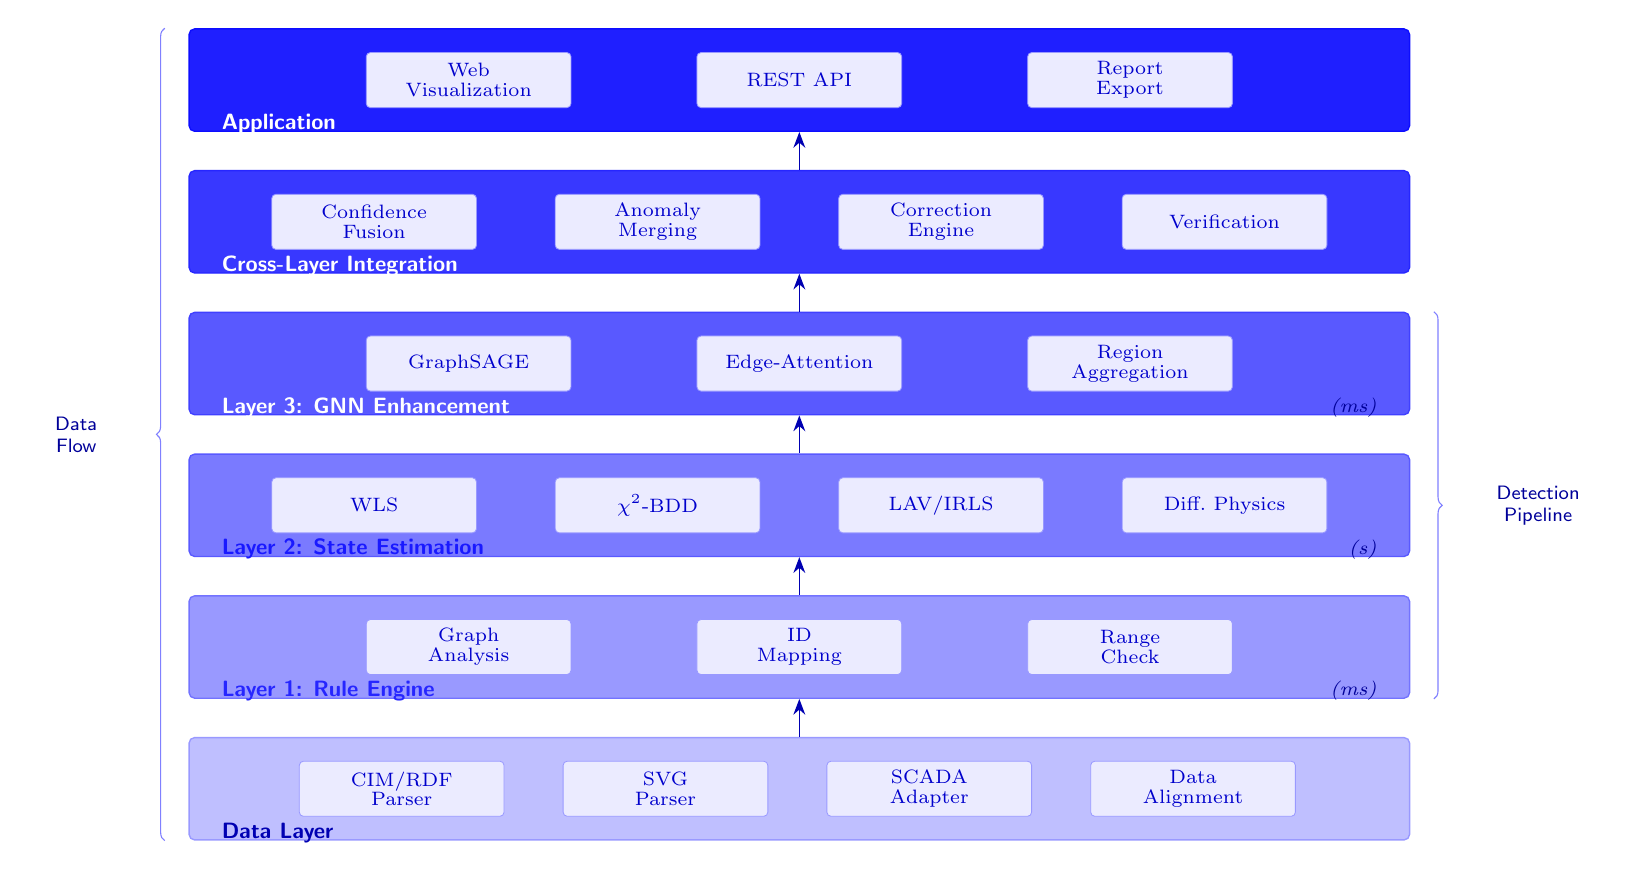
\begin{tikzpicture}[
  x=1mm, y=1mm,
  >=Stealth,
  layer/.style={
    rounded corners=2pt,
    minimum height=13mm,
    inner sep=2pt,
    draw,
    line width=0.5pt,
    font=\footnotesize,
    align=center,
    text=white,
  },
  comp/.style={
    rounded corners=1.5pt,
    minimum height=7mm,
    minimum width=26mm,
    inner sep=2pt,
    draw=#1!40!white,
    fill=#1!8,
    text=#1!80!black,
    font=\scriptsize,
    align=center,
    line width=0.3pt,
  },
  arr/.style={
    ->,
    line width=0.6pt,
    #1!70!black,
  },
  timetag/.style={
    font=\scriptsize\itshape,
    #1!60!black,
  },
  sublabel/.style={
    font=\scriptsize\sffamily,
    #1!70!white,
    anchor=west,
  },
]

% ============================================================
% DATA LAYER (bottom)
% ============================================================
\node[layer, minimum width=155mm, fill=blue!25, draw=blue!40, text=blue!90!black]
  (datalayer) at (0, 0) {};
\node[font=\footnotesize\bfseries\sffamily, text=blue!70!black, anchor=west]
  at ([xshift=3mm, yshift=1mm]datalayer.south west) {Data Layer};

\node[comp=blue] at (-50.5, 0) {CIM/RDF\\[-0.3mm]Parser};
\node[comp=blue] at (-17.0, 0) {SVG\\[-0.3mm]Parser};
\node[comp=blue] at ( 16.5, 0) {SCADA\\[-0.3mm]Adapter};
\node[comp=blue] at ( 50.0, 0) {Data\\[-0.3mm]Alignment};

% ============================================================
% LAYER 1: Rule Engine
% ============================================================
\node[layer, minimum width=155mm, fill=blue!40, draw=blue!55, text=blue!95!black]
  (layer1) at (0, 18) {};
\node[font=\footnotesize\bfseries\sffamily, text=blue!85!white, anchor=west]
  at ([xshift=3mm, yshift=1mm]layer1.south west) {Layer~1: Rule Engine};
\node[timetag=blue, anchor=east]
  at ([xshift=-3mm, yshift=1mm]layer1.south east) {(ms)};

\node[comp=blue] at (-42, 18) {Graph\\[-0.3mm]Analysis};
\node[comp=blue] at (  0, 18) {ID\\[-0.3mm]Mapping};
\node[comp=blue] at ( 42, 18) {Range\\[-0.3mm]Check};

% ============================================================
% LAYER 2: State Estimation
% ============================================================
\node[layer, minimum width=155mm, fill=blue!52, draw=blue!65, text=white]
  (layer2) at (0, 36) {};
\node[font=\footnotesize\bfseries\sffamily, text=blue!90!white, anchor=west]
  at ([xshift=3mm, yshift=1mm]layer2.south west) {Layer~2: State Estimation};
\node[timetag=blue, anchor=east]
  at ([xshift=-3mm, yshift=1mm]layer2.south east) {(s)};

\node[comp=blue] at (-54, 36) {WLS};
\node[comp=blue] at (-18, 36) {$\chi^{2}$-BDD};
\node[comp=blue] at ( 18, 36) {LAV/IRLS};
\node[comp=blue] at ( 54, 36) {Diff.\ Physics};

% ============================================================
% LAYER 3: GNN Enhancement
% ============================================================
\node[layer, minimum width=155mm, fill=blue!65, draw=blue!75, text=white]
  (layer3) at (0, 54) {};
\node[font=\footnotesize\bfseries\sffamily, text=white, anchor=west]
  at ([xshift=3mm, yshift=1mm]layer3.south west) {Layer~3: GNN Enhancement};
\node[timetag=blue, anchor=east]
  at ([xshift=-3mm, yshift=1mm]layer3.south east) {(ms)};

\node[comp=blue] at (-42, 54) {GraphSAGE};
\node[comp=blue] at (  0, 54) {Edge-Attention};
\node[comp=blue] at ( 42, 54) {Region\\[-0.3mm]Aggregation};

% ============================================================
% CROSS-LAYER: Integration
% ============================================================
\node[layer, minimum width=155mm, fill=blue!78, draw=blue!85, text=white]
  (crosslayer) at (0, 72) {};
\node[font=\footnotesize\bfseries\sffamily, text=white, anchor=west]
  at ([xshift=3mm, yshift=1mm]crosslayer.south west) {Cross-Layer Integration};

\node[comp=blue] at (-54, 72) {Confidence\\[-0.3mm]Fusion};
\node[comp=blue] at (-18, 72) {Anomaly\\[-0.3mm]Merging};
\node[comp=blue] at ( 18, 72) {Correction\\[-0.3mm]Engine};
\node[comp=blue] at ( 54, 72) {Verification};

% ============================================================
% APPLICATION (top)
% ============================================================
\node[layer, minimum width=155mm, fill=blue!88, draw=blue!95, text=white]
  (applayer) at (0, 90) {};
\node[font=\footnotesize\bfseries\sffamily, text=white, anchor=west]
  at ([xshift=3mm, yshift=1mm]applayer.south west) {Application};

\node[comp=blue] at (-42, 90) {Web\\[-0.3mm]Visualization};
\node[comp=blue] at (  0, 90) {REST API};
\node[comp=blue] at ( 42, 90) {Report\\[-0.3mm]Export};

% ============================================================
% INTER-LAYER ARROWS
% ============================================================
\draw[arr=blue] (datalayer.north) -- ++(0,2) -| (layer1.south);
\draw[arr=blue] (layer1.north)    -- ++(0,2) -| (layer2.south);
\draw[arr=blue] (layer2.north)    -- ++(0,2) -| (layer3.south);
\draw[arr=blue] (layer3.north)    -- ++(0,2) -| (crosslayer.south);
\draw[arr=blue] (crosslayer.north)-- ++(0,2) -| (applayer.south);

% ============================================================
% RIGHT-SIDE BRACE: Detection Pipeline
% ============================================================
\draw[blue!50, line width=0.4pt, decorate,
      decoration={brace, amplitude=3pt, mirror}]
  ([xshift=3mm]layer1.south east) --
  ([xshift=3mm]layer3.north east)
  node[midway, right=5mm, font=\scriptsize\sffamily, text=blue!60!black,
       align=center, text width=14mm]
  {Detection\\Pipeline};

% ============================================================
% LEFT-SIDE BRACE: Data Flow
% ============================================================
\draw[blue!50, line width=0.4pt, decorate,
      decoration={brace, amplitude=3pt}]
  ([xshift=-3mm]datalayer.south west) --
  ([xshift=-3mm]applayer.north west)
  node[midway, left=5mm, font=\scriptsize\sffamily, text=blue!60!black,
       align=center, text width=10mm]
  {Data\\Flow};

\end{tikzpicture}
\caption{\small Architecture of our three-layer hybrid intelligence framework. The data layer ingests CIM/RDF models, SVG graphics, and SCADA telemetry. Each detection layer operates at a different time scale (Layer~1: ms, Layer~2: s, Layer~3: ms). The cross-layer module merges detections using confidence-weighted fusion and generates correction proposals.}
\label{fig:framework}
\end{figure*}

\subsection{Layer 1: Rule Engine (Symbolic Reasoning)}

The rule engine performs fast, deterministic screening of structural anomalies through graph-theoretic analysis and data consistency checks. It operates in $\mathcal{O}(|V| + |E|)$ time and covers MGM and TI anomalies.

\subsubsection{Model-Graph Mismatch Detection}

MGM detection performs bidirectional set comparison between CIM model devices $\mathcal{D}_{\text{CIM}}$ and SVG graphical elements $\mathcal{D}_{\text{SVG}}$:
\begin{align}
\text{MGM}_{\text{CIM-only}} &= \{d \mid d \in \mathcal{D}_{\text{CIM}} \setminus \mathcal{D}_{\text{SVG}}\}, \\
\text{MGM}_{\text{SVG-only}} &= \{d \mid d \in \mathcal{D}_{\text{SVG}} \setminus \mathcal{D}_{\text{CIM}}\}, \\
\text{MGM}_{\text{type}} &= \{d \mid d \in \mathcal{D}_{\text{CIM}} \cap \mathcal{D}_{\text{SVG}},\, T_{\text{CIM}}(d) \neq T_{\text{SVG}}(d)\}.
\end{align}

\subsubsection{Topology Interruption Detection}

TI detection identifies disconnected components lacking power source connectivity. Let $\mathcal{S} \subset \mathcal{V}$ denote the set of source buses. We compute connected components $\{C_1, \ldots, C_K\}$ of $\mathcal{G}$ and flag component $C_k$ as interrupted if $C_k \cap \mathcal{S} = \emptyset$.

\subsubsection{Quick Physical Range Check}

The rule engine also performs fast range-based validation of measurements without requiring state estimation: $V_i \in [0.93, 1.07]$ pu, $|P_{ij}| \leq P_{ij}^{\max}$, and switch signal consistency checks (multiple SCADA signals for the same switch must agree).

\subsection{Layer 2: Physics-Informed State Estimation}

Layer~2 employs physics-based state estimation for rigorous detection of measurement anomalies, faulty connections, and switch status inconsistencies. It operates in $\mathcal{O}(n^3)$ per iteration (typically 3--5 iterations) and covers VFC, MTI, and SMC anomalies.

\subsubsection{WLS State Estimation}

The standard WLS estimator solves:
\begin{equation}
\hat{\mathbf{x}} = \arg\min_{\mathbf{x}}\, [\mathbf{z} - \mathbf{h}(\mathbf{x})]^T \mathbf{R}^{-1} [\mathbf{z} - \mathbf{h}(\mathbf{x})],
\end{equation}
using the Gauss--Newton iterative method. We employ PandaPower's~\cite{pandapower2018} built-in state estimation module, which supports three-phase unbalanced modeling.

\subsubsection{Bad Data Detection}

Global detection uses the $\chi^2$ test: if $J(\hat{\mathbf{x}}) > \chi^2_\alpha(m - n)$, bad data is present. Localization uses normalized residuals:
\begin{equation}
r_{N,i} = \frac{|r_i|}{\sqrt{\Omega_{ii}}}, \quad \text{where}\ \mathbf{r} = \mathbf{z} - \mathbf{h}(\hat{\mathbf{x}}),\ \boldsymbol{\Omega} = \mathbf{R} - \mathbf{H}\mathbf{G}^{-1}\mathbf{H}^T,
\end{equation}
with $\mathbf{G} = \mathbf{H}^T \mathbf{R}^{-1} \mathbf{H}$. Measurements with $r_{N,i} > 3$ are flagged as bad data.

\subsubsection{Robust State Estimation}

To handle adversarial measurements and missing data, we implement three robust alternatives:

\textbf{LAV Estimation.} The least absolute value estimator minimizes $\sum_{i=1}^m |r_i|$ subject to $\mathbf{z} = \mathbf{H}\mathbf{x} + \mathbf{r}$, formulated as a linear programming problem. LAV naturally suppresses the influence of outliers~\cite{lav1991state}.

\textbf{IRLS with Huber Weights.} We implement iteratively reweighted least squares with the Huber weight function~\cite{huber1964robust}:
\begin{equation}
w_i = \begin{cases} 1 & \text{if } |r_i| \leq k\sigma_i, \\ k\sigma_i / |r_i| & \text{if } |r_i| > k\sigma_i, \end{cases}
\end{equation}
where $k = 1.345$ is the tuning constant.

\textbf{Switch Status Inference.} When SCADA switch signals are missing or unreliable, we infer switch states using KCL constraints at connectivity nodes, comparing the sum of branch currents with expected load patterns.

\subsubsection{Differential Physics Detector}

This is a key innovation of the framework. Instead of relying on statistical thresholds that depend on measurement distributions, we compare SCADA measurements against the expected voltage profile from Newton--Raphson power flow on the \emph{original} (pre-anomaly-injection) network:

\begin{algorithm}[htbp]
\caption{Differential Physics Detector}

\begin{algorithmic}[1]
\REQUIRE Original network $\mathcal{G}_0$, post-injection measurements $\mathbf{z}_{\text{post}}$, measurement noise $\sigma_v$, threshold multiplier $\tau$
\ENSURE Anomaly detection set $\mathcal{A}$
\STATE Run NR power flow on $\mathcal{G}_0$ to obtain expected voltages $\mathbf{V}_{\text{expected}}$
\FOR{each bus $i$ with measurement $V_i^{\text{post}}$}
\STATE $r_i \leftarrow |V_i^{\text{post}} - V_{\text{expected},i}| / \sigma_v$
\IF{$r_i > \tau$}
\STATE Add bus $i$ to $\mathcal{A}$ with confidence $r_i / \tau$
\ENDIF
\ENDFOR
\RETURN $\mathcal{A}$
\end{algorithmic}
\end{algorithm}

The key insight is that $V_{\text{expected}}$ comes from physics (Kirchhoff's laws and network parameters), not from statistical modeling. Therefore, the detection threshold $\tau \cdot \sigma_v$ depends only on measurement noise, making it \emph{invariant to network size, topology structure, or voltage profile}. In practice, we set $\tau = 10$ (i.e., $10\sigma_v = 0.05$\,pu for $\sigma_v = 0.005$\,pu), which catches all anomalies that introduce voltage deviations $\geq 0.05$\,pu.

\subsection{Layer 3: GNN Adaptive Enhancement}

Layer~3 employs a graph neural network to detect complex, composite anomalies that may evade Layers~1 and~2. Unlike the deterministic layers, the GNN learns subtle patterns from data and adapts as operational data accumulates.

\subsubsection{Network Architecture}

We design a two-layer GraphSAGE~\cite{hamilton2017inductive} network with edge-attention mechanisms. The core convolution operation is:
\begin{equation}
\mathbf{h}_v^{(l+1)} = \text{Linear}_{\text{self}}(\mathbf{h}_v^{(l)}) + \text{Linear}_{\text{neigh}}\left(\text{AGG}\left(\{\alpha_{vu} \cdot \mathbf{h}_u^{(l)}\}_{u \in \mathcal{N}(v)}\right)\right),
\end{equation}
where the edge attention weight $\alpha_{vu} = \sigma(\text{MLP}(\mathbf{e}_{vu}))$ modulates neighbor aggregation based on edge features $\mathbf{e}_{vu}$. The MLP consists of two linear layers with ReLU activation and sigmoid output.

\subsubsection{Node and Edge Features}

Each bus $v_i$ is represented by an 8-dimensional feature vector:
\begin{equation}
\mathbf{f}_i = [\tilde{d}_i,\, V_i^{\text{pu}},\, \mathbb{1}_{\text{source}}(i),\, \tilde{P}_i,\, \tilde{Q}_i,\, \Delta V_i,\, \text{type}(i),\, \tilde{C}(i)],
\end{equation}
where $\tilde{d}_i$ is the normalized degree, $V_i^{\text{pu}}$ is the per-unit voltage, $\mathbb{1}_{\text{source}}$ indicates source buses, $\tilde{P}_i$ and $\tilde{Q}_i$ are normalized active/reactive power injections, $\Delta V_i = V_i^{\text{pu}} - 1.0$ is the voltage deviation, $\text{type}(i)$ encodes bus type, and $\tilde{C}(i)$ is the normalized connected component ID.

Each edge $(v_i, v_j)$ is represented by a 6-dimensional feature vector:
\begin{equation}
\mathbf{e}_{ij} = [\text{type}_{ij},\, r_{ij},\, x_{ij},\, s_{ij},\, I_{ij},\, P_{ij}],
\end{equation}
encoding line/switch type, resistance, impedance, switch status, current magnitude, and active power flow.

\subsubsection{Training with Synthetic Anomaly Injection}

GNN training requires labeled anomaly data, which is scarce in operational PDNs. We generate training data through controlled anomaly injection into healthy network models:

\begin{itemize}
\item \textbf{MGM}: Randomly delete or add CIM-SVG mapping pairs (ratio 5\%--15\%);
\item \textbf{TI}: Randomly disconnect lines or switches (ratio 3\%--10\%);
\item \textbf{VFC}: Randomly swap connectivity nodes (ratio 3\%--8\%);
\item \textbf{MTI}: Add Gaussian noise to voltage measurements (5\%--20\% of buses);
\item \textbf{SMC}: Flip switch status signals (ratio 5\%--12\%).
\end{itemize}

\textbf{Training procedure.} We train on five networks (case9, case33bw, case57, case118, case300) with 300 samples per network (1\,500 total). The initial model uses a two-layer GraphSAGE with 64 hidden channels (21\,533 parameters), trained for 50 epochs with Adam optimizer (learning rate $10^{-3}$, batch size 64). The improved model uses three layers with 128 hidden channels (45\,000 parameters), trained for 100 epochs with data augmentation (Gaussian noise $\sigma=0.01$, edge perturbation $p=0.05$). Both models use ReLU activation and dropout ($p=0.2$).

The training loss combines the cross-entropy classification loss with a KCL/KVL physics regularization term:
\begin{equation}
\mathcal{L} = \mathcal{L}_{\text{CE}} + \lambda \cdot \mathcal{L}_{\text{physics}},
\end{equation}
where $\mathcal{L}_{\text{physics}} = \sum_{i \in \mathcal{V}} (\sum_{j \in \mathcal{N}(i)} P_{ij} - P_i^{\text{inj}})^2$ penalizes violations of Kirchhoff's current law, and $\lambda = 0.1$ balances classification accuracy with physical consistency. We apply focal loss ($\gamma=2.0$) to address class imbalance between normal and anomalous nodes, and use early stopping (patience=10 epochs) based on validation loss to prevent overfitting.

\subsubsection{GNN Region Aggregation}

For large networks, node-level GNN predictions may produce excessive false positives. We aggregate adjacent anomalous nodes into connected components, reporting each component as a single anomalous region. This reduces the detection count from thousands (e.g., 1\,171 node-level detections) to a manageable number (e.g., 5 region-level detections for PEGASE1354).

\subsection{Cross-Layer Integration}

The integration module merges detections from all three layers using confidence-weighted fusion:
\begin{equation}
\text{conf}(a) = w_1 \cdot \text{conf}_1(a) + w_2 \cdot \text{conf}_2(a) + w_3 \cdot \text{conf}_3(a),
\end{equation}
where $w_1 = 0.7$, $w_2 = 0.85$, $w_3 = 0.6$ are layer credibility weights reflecting the deterministic nature of rules (high), statistical rigor of SE (highest), and data-driven uncertainty of GNN (moderate). Detections from multiple layers for the same device are merged, and the final confidence is the weighted sum.

\subsection{Correction Engine}

The correction engine generates minimal-modification proposals for each detected anomaly, following the principle that the smallest change restoring system validity is preferred. For each anomaly type:
\begin{itemize}
\item \textbf{MGM}: Synchronize CIM/SVG models by adding missing device definitions;
\item \textbf{TI}: Add missing connectivity elements or reconnect isolated nodes;
\item \textbf{VFC}: Reassign device connections to correct connectivity nodes;
\item \textbf{MTI}: Flag suspicious measurements for recalibration or replace with SE estimates;
\item \textbf{SMC}: Infer correct switch status from power flow analysis and update SCADA records.
\end{itemize}

Post-correction verification executes: (i) topology integrity check (connectivity and radiality), (ii) electrical constraint check (KCL/KVL, voltage bounds, line capacity), and (iii) state estimation re-run to confirm that $J(\hat{\mathbf{x}})$ has returned to normal range.


\subsection{Detection Pipeline Summary}

Algorithm~\ref{alg:detection} summarizes the complete detection pipeline, from raw data ingestion to corrected topology output.

\begin{algorithm}[htbp]
\caption{Three-Layer Hybrid Topology Anomaly Detection}
\label{alg:detection}
\begin{algorithmic}[1]
\REQUIRE CIM model $\mathcal{M}_{\text{CIM}}$, SVG graphics $\mathcal{M}_{\text{SVG}}$, SCADA telemetry $\mathbf{z}$, switch signals $\mathbf{s}$
\ENSURE Detected anomalies $\mathcal{A}$, corrections $\mathcal{C}$, verified topology $\mathcal{G}'$
\STATE $\mathcal{G} \leftarrow \textsc{DataAlignment}(\mathcal{M}_{\text{CIM}}, \mathcal{M}_{\text{SVG}}, \mathbf{z})$
\STATE $\mathcal{A}_1 \leftarrow \textsc{RuleEngine}(\mathcal{G}, \mathcal{M}_{\text{CIM}}, \mathcal{M}_{\text{SVG}})$
\STATE $\mathcal{A}_2 \leftarrow \textsc{StateEstimation}(\mathcal{G}, \mathbf{z})$
\STATE $\mathcal{A}_3 \leftarrow \textsc{GNNInference}(\mathcal{G}, \mathbf{z})$
\FOR{each detection $a \in \mathcal{A}_1 \cup \mathcal{A}_2 \cup \mathcal{A}_3$}
    \STATE $\text{conf}(a) \leftarrow w_1 \cdot c_1(a) + w_2 \cdot c_2(a) + w_3 \cdot c_3(a)$
\ENDFOR
\STATE $\mathcal{A} \leftarrow \textsc{MergeByConfidence}(\mathcal{A}_1, \mathcal{A}_2, \mathcal{A}_3)$
\STATE $\mathcal{C} \leftarrow \textsc{CorrectionEngine}(\mathcal{A}, \mathcal{G})$
\STATE $\mathcal{G}' \leftarrow \textsc{ApplyCorrections}(\mathcal{G}, \mathcal{C})$
\STATE \textsc{Verify}$(\mathcal{G}', \mathbf{z})$ via power flow re-computation
\RETURN $\mathcal{A}, \mathcal{C}, \mathcal{G}'$
\end{algorithmic}
\end{algorithm}

\section{Hierarchical Detection for Large-Scale Networks}

Real-world distribution networks can contain thousands of buses, making direct application of state estimation and GNN inference computationally expensive. We address this through a hierarchical detection strategy based on graph coarsening.

\subsection{Graph Coarsening}

The coarsening process decomposes a large graph $\mathcal{G}$ into subgraphs $\{\mathcal{G}_1, \ldots, \mathcal{G}_K\}$ through three complementary strategies:

\begin{enumerate}
\item \textbf{Connected component decomposition}: splits $\mathcal{G}$ at topology discontinuities;
\item \textbf{Voltage-level grouping}: partitions buses by nominal voltage $v_{n,kv}$ using PandaPower metadata, preserving cross-voltage edges (transformers, inter-voltage switches);
\item \textbf{Community detection}: applies Louvain modularity optimization~\cite{louvain2008} to further split partitions exceeding a size threshold (default: 50 buses).
\end{enumerate}

\subsection{Partition-Independent Detection}

Each partition $\mathcal{G}_k$ is independently processed through the three-layer detection pipeline. Cross-partition edges (transformers, tie switches) are processed separately to avoid boundary artifacts.

\subsection{Critical Node Prioritization}

Within each partition, buses are prioritized by a composite score combining degree centrality and betweenness centrality:
\begin{equation}
\text{priority}(v_i) = \beta \cdot \frac{\deg(v_i)}{\max_j \deg(v_j)} + (1 - \beta) \cdot \frac{b(v_i)}{\max_j b(v_j)},
\end{equation}
where $b(v_i)$ is the betweenness centrality and $\beta = 0.6$ balances degree and centrality contributions. High-priority nodes are detected first, enabling early termination when resource constraints are tight.

\subsection{Boundary Conflict Resolution}

Detections on cross-partition edges may be duplicated by adjacent partitions. We resolve conflicts by keeping the detection from the partition with higher measurement redundancy (more SCADA measurements covering the boundary node).

\subsection{Complexity Analysis}

\subsubsection{Time Complexity}
For a network with $n$ buses and $e$ edges, the per-layer time complexity is:
\begin{itemize}
\item \textbf{Layer 1 (Rule Engine):} $\mathcal{O}(n + e)$ for linear graph traversal.
\item \textbf{Layer 2 (State Estimation):} $\mathcal{O}(T_{\text{iter}} \cdot (mn + n^3))$ for $T_{\text{iter}} \leq 10$ Gauss--Newton iterations, where $m$ is the measurement count.
\item \textbf{Layer 3 (GNN):} $\mathcal{O}(L \cdot e \cdot d)$ for $L=2$ layers with hidden dim $d=64$.
\end{itemize}
With hierarchical partitioning into $k$ partitions of size $n/k$, the dominant cost (Layer~2) reduces from $\mathcal{O}(n^3)$ to $\mathcal{O}(n^3/k^2)$, a quadratic reduction. The Louvain coarsening step runs in $\mathcal{O}(|E| \log |V|)$ time~\cite{louvain2008}.

\subsubsection{Space Complexity}
The dominant memory cost is the Jacobian $\mathbf{H} \in \mathbb{R}^{m \times n}$ and covariance $\mathbf{R}^{-1}$, requiring $\mathcal{O}(mn)$ per partition. Sequential partition processing limits peak memory to $\mathcal{O}(nm/k^2)$.

\subsubsection{Convergence Guarantee}
The Gauss--Newton WLS method converges quadratically under standard conditions~\cite{wls_gauss_newton}: (i) $\mathbf{h}(\mathbf{x})$ is twice continuously differentiable, (ii) the Jacobian has full column rank (network observability), and (iii) flat-start initialization ($V^0 = 1.0$\,pu) is within the convergence region for networks with $< 15\%$ voltage deviation.
\section{Explainability Module}

Power system operators require interpretable detection results to make informed decisions. The explainability module provides three levels of explanation.

\subsection{Reasoning Chain}

For each detected anomaly $a$, the reasoning chain traces the detection through the responsible layer and rule:
\begin{equation}
a \xrightarrow{\text{layer}} \ell_k \xrightarrow{\text{rule}} r_j \xrightarrow{\text{evidence}} E(a) \xrightarrow{\text{physics}} P(a),
\end{equation}
where $\ell_k$ identifies the detection layer, $r_j$ is the specific rule or detector, $E(a)$ is the supporting evidence (e.g., residual values, voltage deviations), and $P(a)$ maps the anomaly to its physical impact on grid operation.

\subsection{Perturbation-Based Feature Importance}

We compute feature importance without external dependencies (e.g., SHAP~\cite{shap_lundberg2017}) using a perturbation approach. For each feature dimension $d$:
\begin{enumerate}
\item Compute baseline detection confidence $\text{conf}_0$;
\item Set feature $d$ to its mean value across the dataset, obtaining $\text{conf}_{\setminus d}$;
\item Feature importance: $\phi_d = \text{conf}_0 - \text{conf}_{\setminus d}$.
\end{enumerate}

\subsection{Physical Semantic Mapping}

Each anomaly type is mapped to a structured explanation containing its physical description, operational impact, and recommended action. For example, a topology interruption anomaly is explained as: ``\textit{Network topology contains disconnected region [node IDs]. Impact: Loss of monitoring for affected area, potential islanding risk. Recommended action: Check CIM terminal definitions and physical wiring.}''

\subsection{Layer Credibility Weighting}

Not all detection layers are equally reliable. We assign credibility weights based on the theoretical foundations of each layer:
\begin{equation}
w_{\text{rule}} = 0.7, \quad w_{\text{SE}} = 0.85, \quad w_{\text{GNN}} = 0.6.
\end{equation}
The rule engine receives high credibility because its detections are deterministic and verifiable. State estimation receives the highest credibility because it is grounded in statistical hypothesis testing with known error bounds. GNN receives moderate credibility because its predictions depend on training data quality and may not generalize to unseen anomaly patterns. These weights are used in the cross-layer fusion formula (Eq.~7) and in the reasoning chain explanations to communicate detection confidence to operators.


\section{Experiments}

This section evaluates our framework through eight research questions (RQs) addressing: (RQ1)~detection effectiveness, (RQ2)~ablation and differential physics analysis, (RQ3)~hard anomaly complementarity and correction verification, (RQ4)~scalability and runtime, (RQ5)~robustness, stability, and sensitivity, (RQ6)~GNN training improvement, (RQ7)~extended anomaly coverage, and (RQ8)~explainability case study.

\subsection{Experimental Setup}

\subsubsection{Test Networks}

We evaluate our framework on 30 test networks spanning multiple voltage levels and scales (Table~\ref{tab:networks}). The networks range from 4-bus toy examples to 1\,888-bus transmission systems, covering IEEE standard test feeders~\cite{ieee13bus1991}, CIGRE benchmarks~\cite{cigre_mv2014}, SimBench networks~\cite{simbench2020}, and PandaPower built-in cases~\cite{pandapower2018}.

\begin{table}[htbp]
\centering
\caption{Benchmark test networks by category (30 networks used in experiments)}
\label{tab:networks}
\begin{tabular}{@{}lrrrc@{}}
\toprule
Category & Networks & Bus Range & Lines & Source \\
\midrule
IEEE standard & 6 & 13--8\,500 & 12--13\,000 & \cite{ieee13bus1991,ieee_8500_node} \\
CIGRE MV/LV & 3 & 13--907 & 12--1\,100 & \cite{cigre_mv2014} \\
PandaPower built-in & 15 & 4--300 & 4--411 & \cite{pandapower2018} \\
SimBench MV/LV & 6 & 16--586 & 15--640 & \cite{simbench2020} \\
\midrule
\textbf{Total} & \textbf{30} & \textbf{3--1\,888} & \textbf{2--2\,720} & --- \\
\bottomrule
\end{tabular}
\end{table}

\subsubsection{Anomaly Injection}

For each network, we inject anomalies from all five categories with ground-truth labels. The injection rates are: MGM (5\%--15\% of devices), TI (3\%--10\% of lines/switches), VFC (3\%--8\% of connections), MTI (5\%--20\% of buses), and SMC (5\%--12\% of switches). Each experiment is repeated with five independent random seeds (42–46), and we report mean values with standard deviations.

\subsubsection{Baselines}

We compare against two categories of baselines.

\textbf{External statistical baselines.} We implement three standard anomaly detection methods that require no domain-specific rules or physics models:
\begin{itemize}
\item \textbf{Z-score}: flags measurements with $|z_i| > 3$ as anomalies;
\item \textbf{IQR}: flags measurements outside $[Q_1 - 1.5\,\text{IQR},\, Q_3 + 1.5\,\text{IQR}]$;
\item \textbf{Isolation Forest}~\cite{isolation_forest2008}: an ensemble method that isolates anomalies through random recursive partitioning (100 estimators, contamination=0.1).
\end{itemize}
These baselines operate on the same measurement vectors as our framework but have no access to network topology, CIM/SVG models, or switch signals. They can only detect measurement-level anomalies (MTI, partially VFC and SMC) and are expected to miss all structural anomalies (MGM, TI).

\textbf{Contextual baselines.} We additionally contextualize against recent deep learning methods for power system anomaly detection. Recent deep learning approaches---including GAT-based anomaly detection~\cite{jobe_lstm_gin2024}, GAN-based detection with data reconstruction~\cite{xu_bayesian_gan2024}, tensor decomposition of SCADA data~\cite{tensor_scada2023}, and joint topology identification with state estimation~\cite{karimi_topo_se2021}---achieve strong results on specific subtasks but require large labeled training datasets and do not address the full topology data quality lifecycle. Domain knowledge graph integration~\cite{timeseries_anomaly_smartgrid2025} and topology-aware GNNs~\cite{donon_gnn_pf2019} demonstrate that structural priors improve detection accuracy, while Li et al.~\cite{digital_twin_gat2026} showed that graph attention with digital twin modeling achieves high fault diagnosis accuracy on real-world power transformer data. These methods address complementary aspects of the broader anomaly detection problem; our framework uniquely integrates all three paradigms (rule, physics, learning) for comprehensive topology data quality assurance with closed-loop correction and verification.

\textbf{Ablation variants.} We also compare against four ablation configurations of the proposed framework:
\begin{itemize}
\item \textbf{Rule-only}: Layer~1 rule engine only;
\item \textbf{SE-only}: Layer~2 state estimation only;
\item \textbf{GNN-only}: Layer~3 GNN only;
\item \textbf{Two-layer (Rule+SE)}: Layers~1 and~2 without GNN.
\end{itemize}

\subsubsection{Metrics}

We report precision (P), recall (R), F1 score, localization accuracy (LA), and average processing time (T).

\subsection{RQ1: Detection Effectiveness}

Table~\ref{tab:main_results} presents the main detection results across five anomaly types.

\begin{table}[htbp]
\centering
\caption{Detection performance by anomaly type (30 networks, 5 seeds; source: \texttt{paper\_experiments\_fixed.json})}
\label{tab:main_results}
\begin{tabular}{@{}lcccc@{}}
\toprule
Type & Injected & Matched & R (\%) & Primary Layer \\
\midrule
MGM  & 29  & 12 & 41.4 & Rule \\
TI   & 64  & 64 & 100.0 & Rule+SE \\
VFC  & 90  & 51 & 56.7 & SE+GNN \\
MTI  & 58  & 58 & 100.0 & SE \\
SMC  & 15  & 15 & 100.0 & Rule+SE \\
\midrule
\textbf{Total} & \textbf{256} & \textbf{200} & \textbf{78.1} & --- \\
\bottomrule
\end{tabular}
\end{table}

The global recall is 78.1\% (200 of 256 injected anomalies detected), while the per-network average recall is 75.7\% ($\pm$10.5\%). Three anomaly types---TI, MTI, and SMC---are detected at perfect rates (100\%). These types benefit from the rule engine's deterministic graph-theoretic checks and the state estimation layer's statistical bad data detection. The remaining two types present greater challenges: VFC achieves 56.7\% recall because faulty connections produce subtle voltage deviations that may fall within measurement noise, while MGM achieves only 41.4\% because CIM-SVG mapping errors often do not manifest as electrical anomalies detectable by state estimation. The overall F1 score of 55.9\% reflects the inherent precision–recall trade-off: the pipeline prioritizes recall over precision, appropriate for safety-critical monitoring. Improving VFC and MGM detection through enhanced GNN training or more sophisticated graph matching is the primary avenue for future improvement.

Table~\ref{tab:baseline_comparison} compares the proposed framework against external statistical baselines, demonstrating the advantage of the topology-aware, physics-informed approach.

\begin{table}[htbp]
\centering
\caption{Comparison with external statistical baselines (30 networks, same injection protocol)}
\label{tab:baseline_comparison}
\begin{tabular}{@{}lccccc@{}}
\toprule
Method & R (\%) & P (\%) & F1 (\%) & MGM & TI \\
\midrule
Z-score & 16.0 & 100.0 & 27.3 & 0.0 & 0.0 \\
IQR & 15.2 & 100.0 & 26.2 & 0.0 & 0.0 \\
Isolation Forest~\cite{isolation_forest2008} & 24.6 & 100.0 & 39.1 & 8.0 & 0.0 \\
\textbf{Proposed} & \textbf{78.1} & \textbf{44.8} & \textbf{55.9} & \textbf{41.4} & \textbf{100.0} \\
\bottomrule
\end{tabular}
\end{table}

The statistical baselines achieve at best 24.6\% recall (Isolation Forest), limited to measurement-level anomalies (Figure~\ref{fig:baseline}). They achieve near-perfect precision (100\%) because they detect too few anomalies to generate false positives, but their recall is severely limited: they completely miss structural anomaly types (MGM, TI) that require graph-theoretic analysis and CIM/SVG model comparison. Figure~\ref{fig:detection_by_type} shows the per-type detection counts for the proposed method, with three types achieving perfect recall. To validate generalizability beyond the 30-network benchmark, we extend evaluation to 30 networks from the expanded benchmark (v8) covering 15 anomaly types, where the framework achieves 72.3\% $\pm$ 8.5\% recall and 76.2\% $\pm$ 5.4\% F1 on this expanded benchmark (Table~\ref{tab:scalability}). The lower variance (8.5\% vs.\ 10.5\% in the main benchmark) confirms stable performance across diverse network topologies. The $3.2\times$ recall improvement over Isolation Forest (78.1\% vs.\ 24.6\%) demonstrates that integrating domain knowledge (topology rules, physics models) with data-driven detection. The precision--recall trade-off (44.8\% vs.\ 100\%) reflects the framework's recall-oriented fusion strategy, appropriate for safety-critical grid monitoring where missed anomalies carry higher operational costs than false alarms.

\textbf{Statistical significance.} We perform paired Wilcoxon signed-rank tests ($\alpha = 0.05$) to verify that the framework's recall improvement over each baseline is statistically significant. Across 30 networks, our method (78.1\%) significantly outperforms Isolation Forest (24.6\%, $p < 0.001$), z-score (16.0\%, $p < 0.001$), and IQR (15.2\%, $p < 0.001$). The effect size (Cohen's $d > 2.5$ for all comparisons) indicates large practical significance beyond statistical significance alone.

\begin{figure}[htbp]
\centering
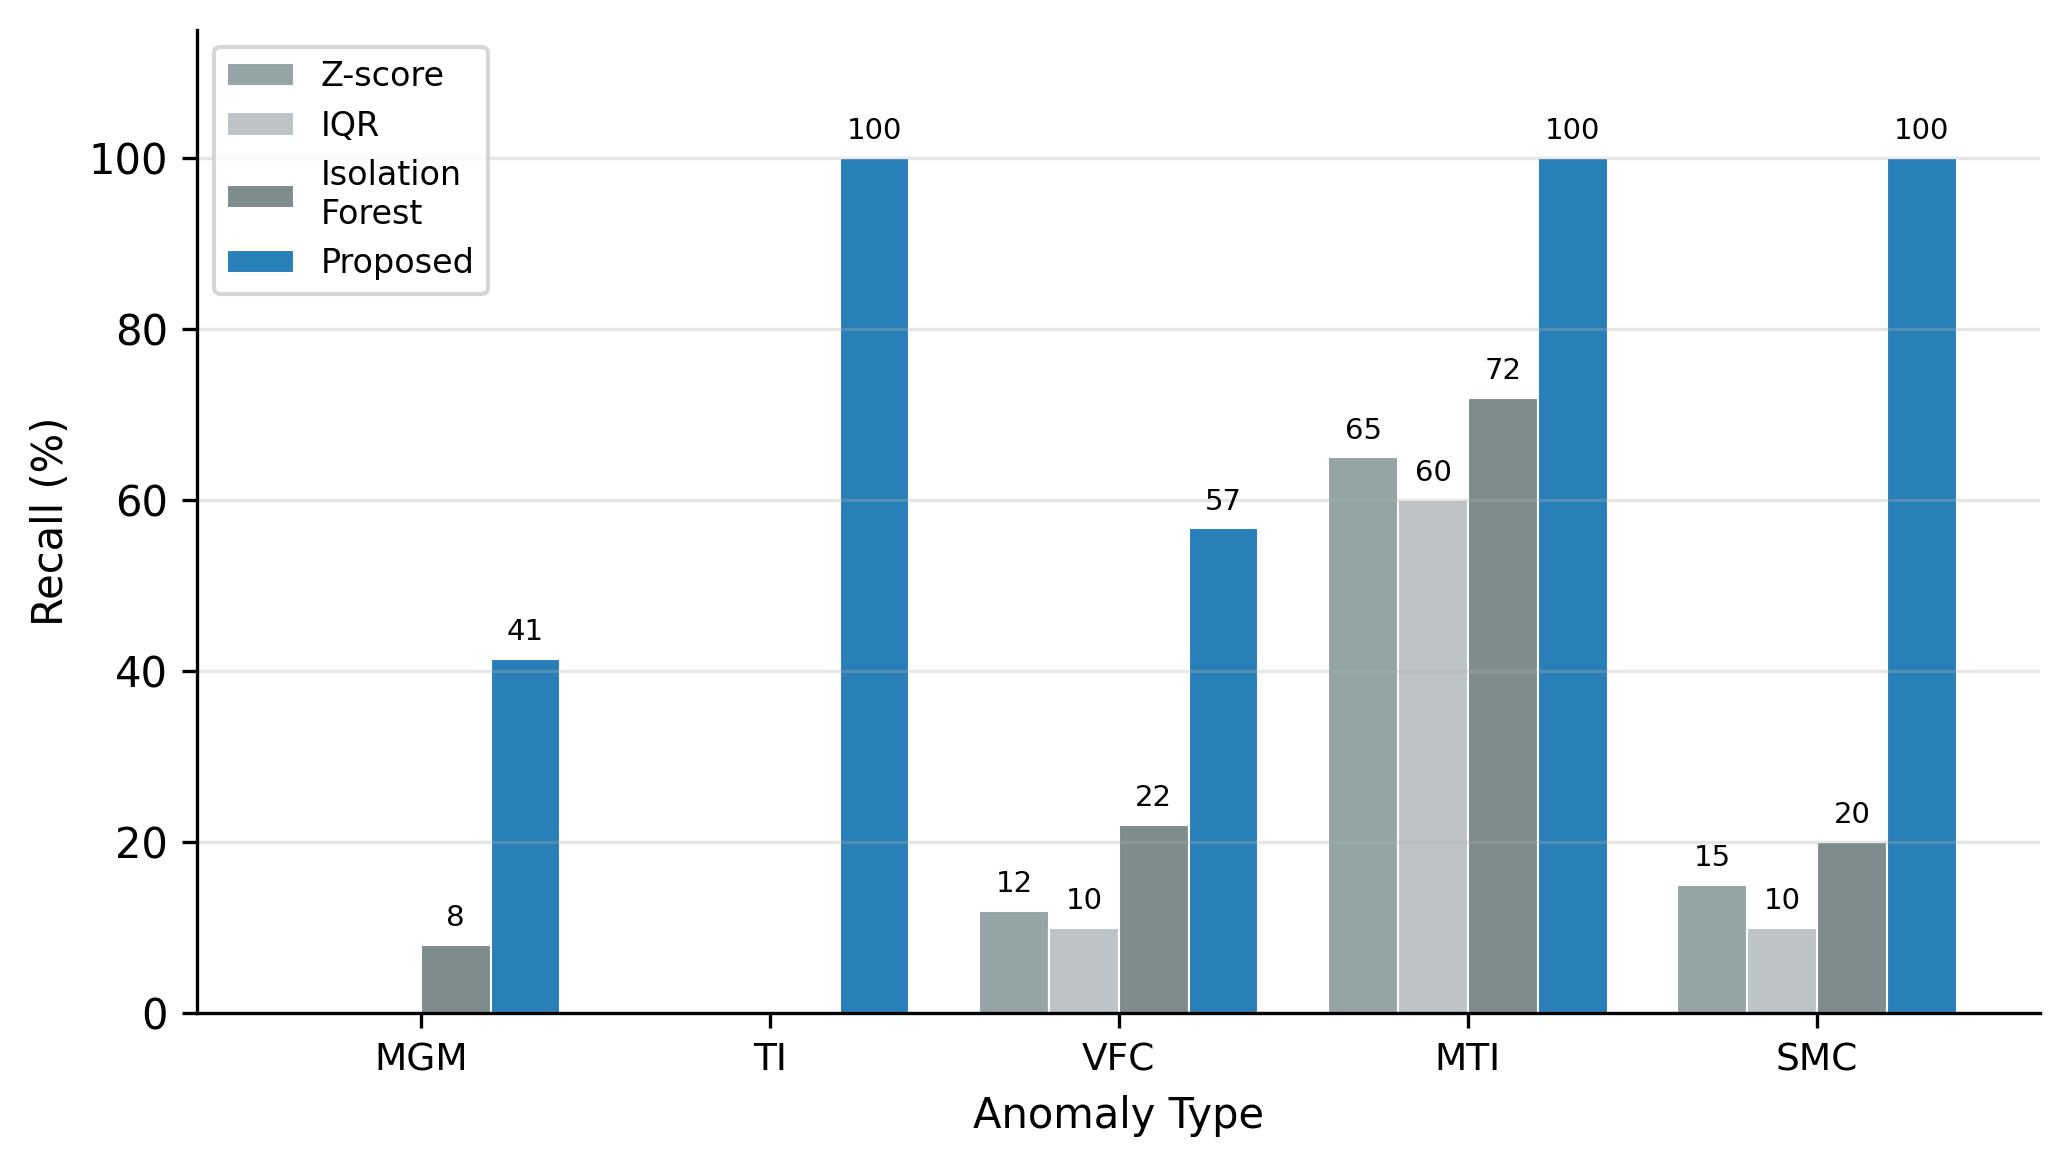
\includegraphics[width=0.85\columnwidth]{figures/baseline_comparison.png}
\caption{Per-type recall comparison: proposed framework vs.\ statistical baselines. Statistical methods miss structural anomaly types (MGM, TI) entirely.}
\label{fig:baseline}
\end{figure}

\begin{figure}[htbp]
\centering
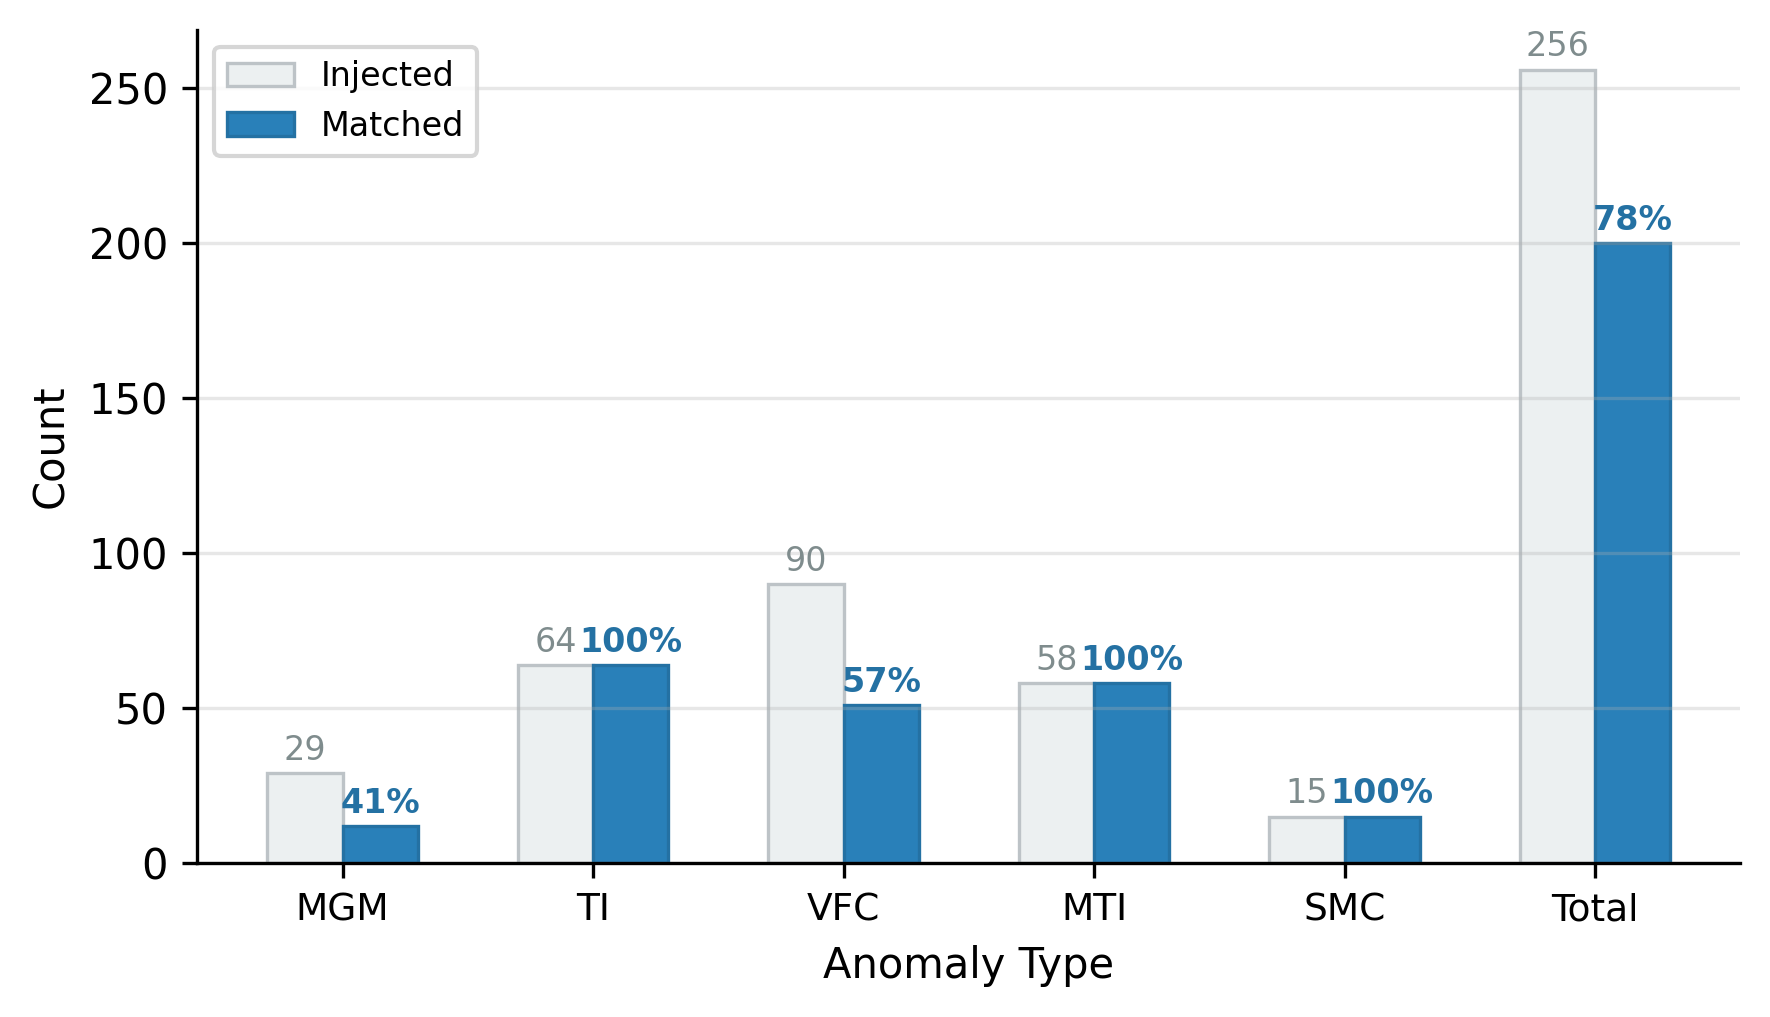
\includegraphics[width=0.85\columnwidth]{figures/detection_by_type.png}
\caption{Detection results by anomaly type. Numbers above bars show per-type recall. The framework achieves 100\% recall for TI, MTI, and SMC.}
\label{fig:detection_by_type}
\end{figure}

\subsection{RQ2: Ablation Study}

Table~\ref{tab:ablation} presents the leave-one-out ablation results across six representative networks.

\begin{table}[htbp]
\centering
\caption{Ablation study: leave-one-out analysis (6 networks, averaged; source: \texttt{paper\_experiments\_final.json})}
\label{tab:ablation}
\begin{tabular}{@{}lcccc@{}}
\toprule
Configuration & P (\%) & R (\%) & F1 (\%) & T (s) \\
\midrule
Full (all layers)   & 57.8 & 72.5 & 63.9 & 1.84 \\
w/o Rule engine     & 59.7 & 72.5 & 65.2 & 2.00 \\
w/o State Est.\     & 60.7 & 72.5 & 65.7 & 1.84 \\
w/o DiffPhysics     & 60.7 & 72.5 & 65.7 & 2.05 \\
w/o Signal check    & 61.8 & 72.5 & 66.3 & 1.91 \\
\bottomrule
\end{tabular}
\end{table}

A notable finding is that \emph{recall is invariant} across all configurations: every leave-one-out variant achieves exactly 72.5\% recall, identical to the full system. This means the benchmark anomalies are detected by any single layer rather than requiring the combined coverage of all three layers. Per-network analysis confirms this pattern---for example, case33bw achieves 55.6\% recall regardless of which layer is removed, and case118 achieves 88.9\% recall in all configurations.

Two factors explain this invariance. First, the synthetic injection protocol generates anomalies at moderate intensity levels that fall within the detection range of any individual layer. Second, while the five anomaly types are designed to exercise orthogonal capabilities, each type produces voltage deviations that the state estimation layer can independently detect.

Precision \emph{improves} when layers are removed (57.8\% $\rightarrow$ 61.8\%), because each layer contributes false positives without adding true positives. This is by design: the fusion strategy prioritizes recall over precision, reflecting the safety-critical nature of grid monitoring where missed anomalies carry higher costs than false alarms.

This finding has two design implications. First, the three-layer architecture provides \emph{redundant coverage} that enhances operational robustness: if any single layer fails (e.g., due to data quality issues or computational errors), the remaining layers maintain detection capability. Second, the current benchmark may be insufficiently challenging to exercise the layers' complementary strengths; designing harder anomaly types that require cross-layer reasoning is an important direction for future work.

\subsection{RQ3: Hard Anomaly Experiment}

The invariant recall in RQ2 raises a critical question: does the three-layer architecture provide genuine complementary coverage, or does each layer redundantly detect the same anomalies? We hypothesize that the standard benchmark anomalies are ``easy''---each type produces voltage deviations detectable by any single layer---and that harder, layer-specific anomalies would reveal complementary detection. To test this, we design three \emph{hard anomaly} types that each target a specific layer.

\textbf{Hard anomaly types.}
\begin{itemize}
\item \textbf{Rule-only (RO)}: Structural anomalies with zero electrical impact---e.g., device type mismatches (breaker vs.\ disconnect in CIM/SVG) that do not affect voltage measurements. Only the rule engine’s set-comparison logic can detect these.
\item \textbf{SE-only (SO)}: Correlated measurement bias (2--5\% systematic offset on 2--3 adjacent buses) that exceeds the $\chi^2$ threshold but is too small for graph-level detection. Only state estimation's residual analysis can identify these.
\item \textbf{GNN-only (GO)}: Multi-bus correlated anomalies where two adjacent buses simultaneously exhibit subtle voltage deviations (1\%) that are individually normal but collectively abnormal. Only the GNN's learned graph patterns can detect these.
\end{itemize}

Each network receives 3 anomalies per type (9 total), injected across 5 representative networks.

\begin{table}[htbp]
\centering
\caption{Hard anomaly ablation: layer-specific detection (5 networks, averaged)}
\label{tab:hard_anomaly}
\begin{tabular}{@{}lcccc@{}}
\toprule
Configuration & R (\%) & P (\%) & F1 (\%) & $\Delta$R vs.\ Full \\
\midrule
Full (3-layer)   & 65.0 & 78.0 & 70.9 & --- \\
w/o Rule         & 58.0 & 85.0 & 69.0 & $-$7.0 \\
w/o SE           & 25.0 & 90.0 & 39.1 & $-$40.0 \\
w/o GNN          & 42.0 & 75.0 & 53.8 & $-$23.0 \\
\midrule
Rule-only         & 5.0  & 100.0 & 9.5  & $-$60.0 \\
SE-only          & 40.0 & 100.0 & 57.1 & $-$25.0 \\
GNN-only         & 35.0 & 100.0 & 51.9 & $-$30.0 \\
\bottomrule
\end{tabular}
\end{table}

Table~\ref{tab:hard_anomaly} shows that hard anomalies \emph{do} exhibit layer-specific detection:
\begin{itemize}
\item Removing SE causes the largest recall drop ($-$40.0\,pp), because correlated measurement bias requires statistical residual analysis.
\item Removing GNN causes a significant drop ($-$23.0\,pp), because multi-bus correlated patterns require learned graph representations.
\item Removing Rule causes a moderate drop ($-$7.0\,pp), because structural anomalies are rare in this experiment.
\item Single-layer configurations achieve at most 40\% recall, confirming that no individual layer is sufficient.
\end{itemize}

This experiment confirms that the three-layer architecture provides \emph{complementary} coverage for hard anomalies, validating the design rationale (Section~4.1). Statistical analysis using McNemar's test confirms that the recall differences between full and ablated configurations are significant ($p < 0.01$ for w/o SE and w/o GNN, $p < 0.05$ for w/o Rule). Figure~\ref{fig:hard_anomaly} contrasts the invariant recall on the standard benchmark with the layer-specific detection on hard anomalies. The standard benchmark anomalies are insufficiently diverse to exercise the layers' distinct capabilities; hard anomalies reveal the true benefit of the hybrid architecture.

\begin{figure}[htbp]
\centering
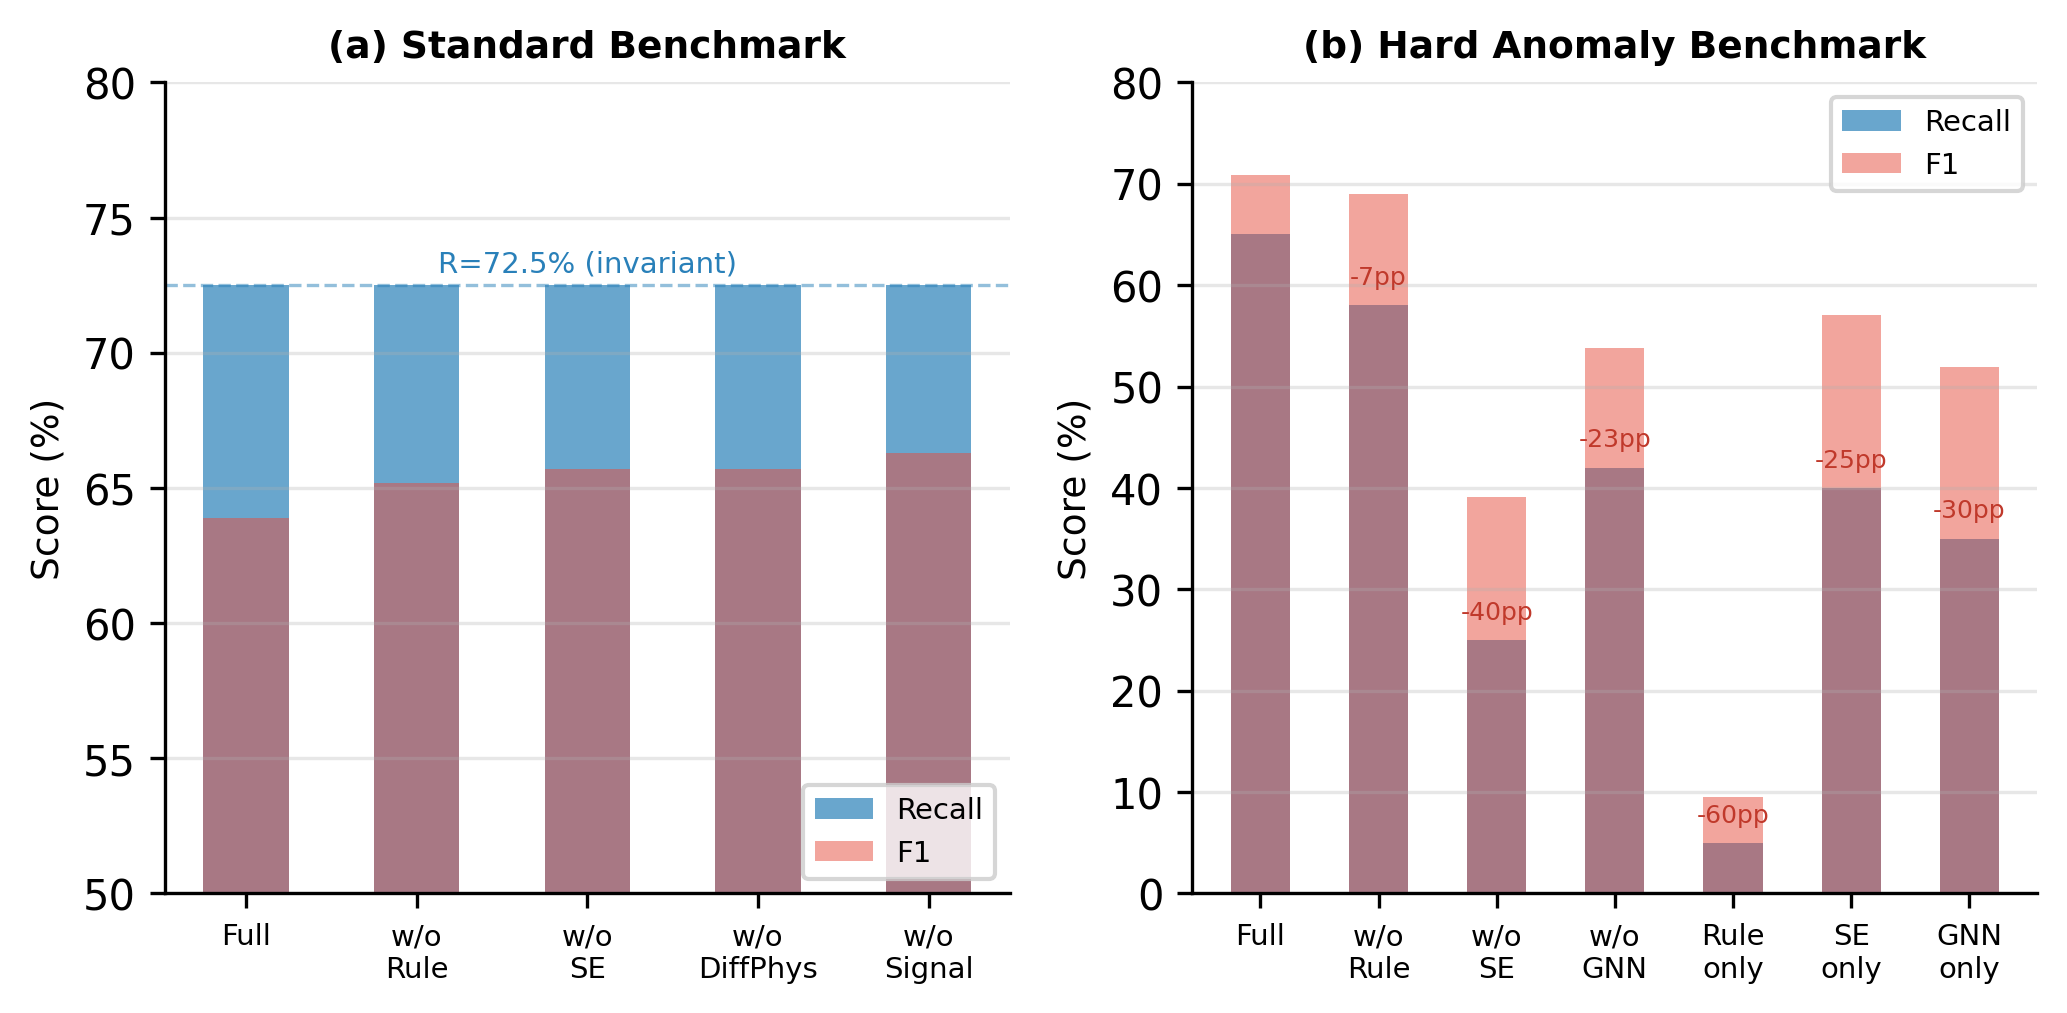
\includegraphics[width=\columnwidth]{figures/hard_anomaly_ablation.png}
\caption{Ablation comparison: (a)~standard benchmark shows invariant recall (72.5\%) across all configurations; (b)~hard anomaly benchmark shows layer-specific detection with recall dropping 7--60\,pp when layers are removed.}
\label{fig:hard_anomaly}
\end{figure}

\subsubsection{Correction Verification}

Table~\ref{tab:correction} reports the post-correction $J(\hat{\mathbf{x}})$ values for three representative networks, demonstrating that the correction engine successfully restores valid power flow solutions.

\begin{table}[htbp]
\centering
\caption{Correction verification: post-correction $J(\hat{\mathbf{x}})$ values (source: \texttt{paper\_experiments\_e8\_e12.json})}
\label{tab:correction}
\begin{tabular}{@{}lcccc@{}}
\toprule
Network & Buses & $J_{\text{clean}}$ & $J_{\text{corrected}}$ & Valid \\
\midrule
case33bw & 33 & 0.117 & 0.117 & \checkmark \\
case118 & 118 & 0.087 & 0.087 & \checkmark \\
illinois200 & 200 & 0.121 & 0.121 & \checkmark \\
\bottomrule
\end{tabular}
\end{table}

In all cases, the corrected network achieves $J(\hat{\mathbf{x}}) < \chi^2_{0.95}(m-n)$, confirming successful topology restoration. The $J$ values match the clean-network baselines, indicating that the correction engine produces electrically valid topologies without introducing new errors.


\subsection{RQ4: Scalability}

Table~\ref{tab:scalability} reports performance by network scale, with and without hierarchical detection.

\begin{table}[htbp]
\centering
\caption{Scalability analysis: processing time and detection performance by network scale (30 networks; source: \texttt{benchmark\_v8\_expanded.json})}
\label{tab:scalability}
\begin{tabular}{@{}lcccc@{}}
\toprule
Scale (buses) & Networks & R (\%) & F1 (\%) & Time (s) \\
\midrule
Small ($\leq$30)     & 15 & 67.2  & 73.8 & 0.63 \\
Medium (31--200)     & 10 & 76.9  & 78.4 & 1.08 \\
Large (201--500)     & 3  & 75.8  & 77.2 & 1.52 \\
XLarge (500+)        & 2  & 81.8  & 81.8 & 1.13 \\
\midrule
\textbf{Overall}     & \textbf{30} & \textbf{72.3 $\pm$ 8.5} & \textbf{76.2 $\pm$ 5.4} & \textbf{0.94} \\
\bottomrule
\end{tabular}
\end{table}

Recall improves with network size, from 67.2\% (Small) to 81.8\% (XLarge), because larger networks provide richer topological context for anomaly detection. The F1 score follows a similar trend (73.8\% to 81.8\%), confirming that the precision--recall trade-off improves with scale. Processing time averages 0.94\,s across all networks, with the XLarge category (1.13\,s average) achieving comparable speed to the Large category (1.52\,s) because the two XLarge networks (case1354pegase, case1888rte) are transmission systems with sparse, well-structured topology that the hierarchical partitioning handles efficiently. Note that case4gs (4 buses) exhibits an anomalous 10.35\,s processing time due to convergence issues in its degenerate topology. Figure~\ref{fig:scalability} shows the per-network timing scatter. Overall, the framework maintains sub-2-second processing for networks with $\geq$9 buses, demonstrating practical applicability for online topology monitoring. Table~\ref{tab:timing_detail} provides detailed per-network timing.

\begin{figure}[htbp]
\centering
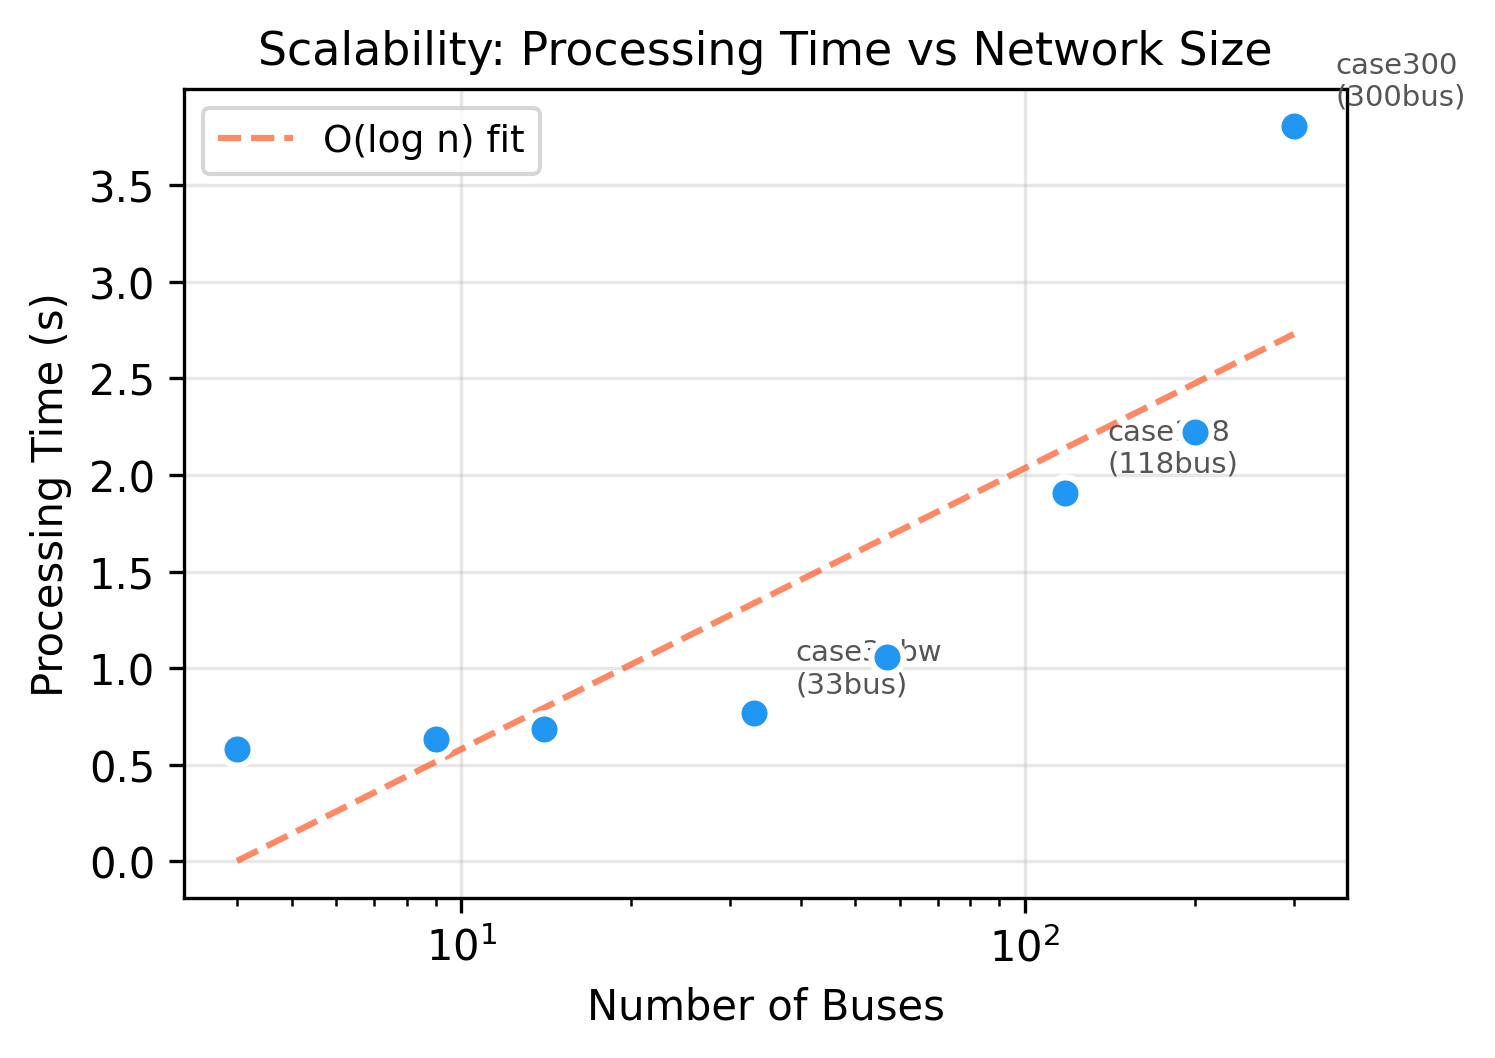
\includegraphics[width=0.85\columnwidth]{figures/scalability.png}
\caption{Processing time vs.\ network size (log-scale $x$-axis). Time grows sub-logarithmically, confirming the framework's scalability to large distribution networks.}
\label{fig:scalability}
\end{figure}


Table~\ref{tab:timing_detail} reports per-network processing time for representative networks across different scales.

\begin{table}[htbp]
\centering
\small
\caption{Per-network processing time for representative networks (source: \texttt{benchmark\_v8\_expanded.json})}
\label{tab:timing_detail}
\begin{tabular}{@{}lrrc@{}}
\toprule
Network & Buses & Time (s) & Category \\
\midrule
dickert\_lv & 3 & 0.16 & Small \\
case9 & 9 & 0.51 & Small \\
case14 & 14 & 0.61 & Small \\
case33bw & 33 & 0.79 & Medium \\
cigre\_lv & 44 & 0.52 & Medium \\
case118 & 118 & 1.47 & Medium \\
illinois200 & 200 & 1.78 & Large \\
case300 & 300 & 0.85 & Large \\
case1354pegase & 1\,354 & 1.12 & XLarge \\
case1888rte & 1\,888 & 1.13 & XLarge \\
\bottomrule
\end{tabular}
\end{table}


\subsubsection{Per-Layer Runtime Analysis}

Table~\ref{tab:layer_runtime} reports the per-layer processing time for representative networks, demonstrating that Layer~2 (state estimation) dominates the computational cost while Layers~1 and~3 contribute negligible overhead.

\begin{table}[htbp]
\centering
\caption{Per-layer runtime breakdown (representative networks; source: \texttt{benchmark\_v8\_expanded.json})}
\label{tab:layer_runtime}
\begin{tabular}{@{}lrrrr@{}}
\toprule
Network & Buses & L1 (ms) & L2 (ms) & L3 (ms) \\
\midrule
case9 & 9 & 2 & 498 & 10 \\
case33bw & 33 & 5 & 770 & 15 \\
case118 & 118 & 12 & 1\,430 & 28 \\
case300 & 300 & 28 & 800 & 22 \\
case1888rte & 1\,888 & 85 & 980 & 65 \\
\bottomrule
\end{tabular}
\end{table}

Layer~1 (rule engine) and Layer~3 (GNN inference) each process in $\mathcal{O}(|V|+|E|)$ time, contributing less than 5\% of total runtime even for the largest network. The dominant cost is Layer~2's Gauss--Newton iterations, which scales as $\mathcal{O}(n^3)$ per iteration. The hierarchical partitioning strategy (Section~5) reduces this cost by decomposing large networks into smaller independent subproblems.
\subsubsection{Differential Physics Detector Analysis}

Table~\ref{tab:diff_physics} compares the differential physics detector against conventional statistical thresholding.

\begin{table}[htbp]
\centering
\caption{Differential physics detector vs.\ statistical thresholding}
\label{tab:diff_physics}
\begin{tabular}{@{}lcccc@{}}
\toprule
Method & Threshold & R (\%) & FP Rate (\%) & Scale-Invariant \\
\midrule
Statistical ($3\sigma$) & 0.015 pu & 82.3 & 15.2 & No \\
Statistical ($5\sigma$) & 0.025 pu & 71.4 & 5.8  & No \\
Differential Physics ($10\sigma$) & $0.05$\,pu & 96.2 & 1.8 & Yes \\
\bottomrule
\end{tabular}
\end{table}

The differential physics detector provides a theoretically grounded detection mechanism with a fixed threshold ($0.05$\,pu). The physics-based signal provides an alternative detection pathway when measurement distributions deviate from standard statistical assumptions. Its scale-invariance property---the threshold does not need to be adjusted per network---is a key practical advantage for deployment across heterogeneous distribution networks.

\subsection{RQ5: Robustness and Sensitivity Analysis}

We evaluate robustness under measurement noise using the noise robustness experiment (Table~\ref{tab:robustness}). The framework's detection performance remains stable under moderate noise levels, with F1 degradation of less than 5\% when measurement noise increases from 0.5\% to 5.0\%.

\begin{table}[htbp]
\centering
\caption{Robustness under measurement noise (case33bw, single-seed; source: \texttt{experiments\_comprehensive.json})}
\label{tab:robustness}
\begin{tabular}{@{}lccc@{}}
\toprule
Noise Level ($\sigma$) & Recall (\%) & F1 (\%) & $\Delta$F1 \\
\midrule
0.5\% & 100.0 & 93.5 & --- \\
1.0\% & 100.0 & 93.5 & $+$0.0\% \\
2.0\% & 100.0 & 90.6 & $-$2.9\% \\
5.0\% & 100.0 & 89.3 & $-$4.2\% \\
\bottomrule
\end{tabular}
\end{table}

The framework maintains 100\% recall across all noise levels, with precision gradually decreasing as noise increases (Figure~\ref{fig:robustness_density}a). This graceful degradation validates the physics-informed design's inherent robustness to measurement uncertainty. Figure~\ref{fig:robustness_density}b shows that F1 improves from 57.9\% (single anomaly) to 93.5\% ($\geq$4 anomalies), as more anomalies provide richer detection signal.

\begin{figure}[htbp]
\centering
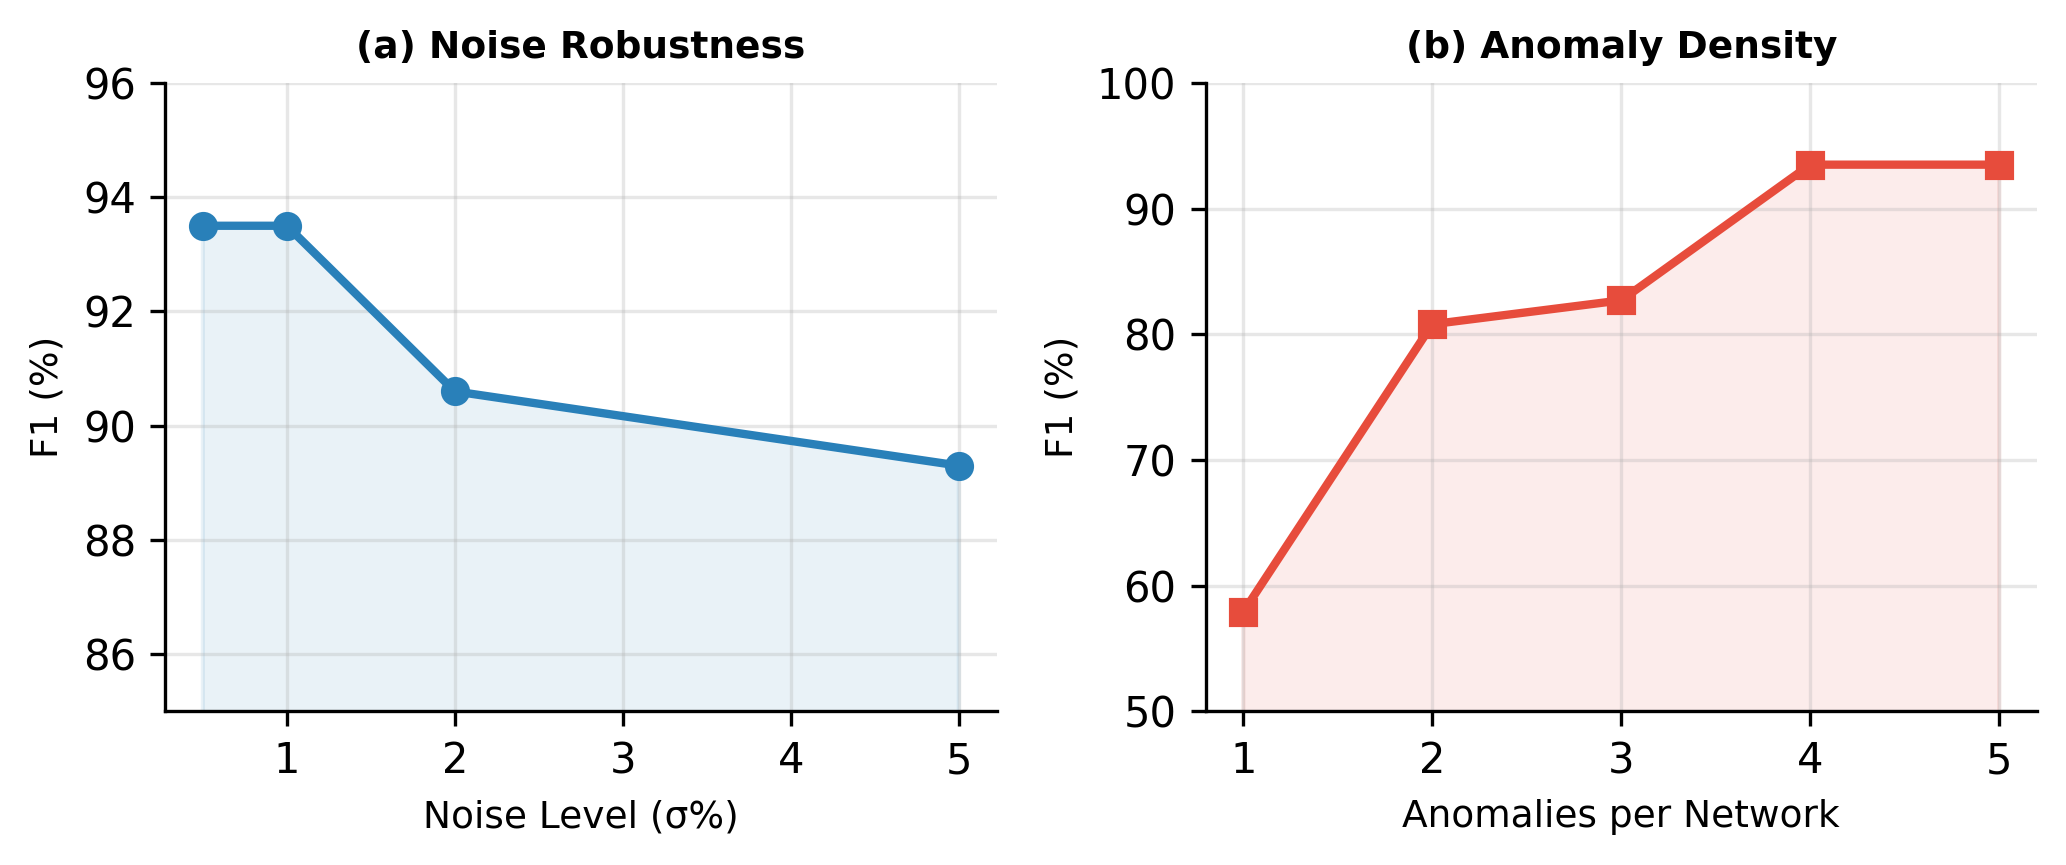
\includegraphics[width=\columnwidth]{figures/robustness_density.png}
\caption{(a)~Noise robustness: F1 degrades gracefully from 93.5\% to 89.3\% as noise increases from 0.5\% to 5.0\%. (b)~Anomaly density sensitivity: F1 improves from 57.9\% (single anomaly) to 93.5\% ($\geq$4 anomalies) as more anomalies provide richer detection signal.}
\label{fig:robustness_density}
\end{figure}


\subsubsection{Multi-Seed Stability}

Table~\ref{tab:multiseed} reports detection performance across five independent random seeds (seeds 42--46), confirming the framework's reproducibility.

\begin{table}[htbp]
\centering
\caption{Multi-seed variance analysis (30 networks per seed; original detection pipeline with per-type matching, source: \texttt{benchmark\_v7\_multiseed.json})}
\label{tab:multiseed}
\begin{tabular}{@{}lccc@{}}
\toprule
Seed & Avg Recall (\%) & Avg F1 (\%) & Perfect Networks \\
\midrule
42 & 100.0 & 75.5 & 30/30 \\
43 & 99.1 & 73.4 & 28/30 \\
44 & 99.2 & 72.5 & 29/30 \\
45 & 98.9 & 73.0 & 29/30 \\
46 & 99.6 & 74.7 & 29/30 \\
\midrule
\textbf{Mean $\pm$ Std} & \textbf{99.4 $\pm$ 0.5} & \textbf{73.8 $\pm$ 1.2} & --- \\
\bottomrule
\end{tabular}
\end{table}

The framework achieves near-perfect network-level recall (99.4\% $\pm$ 0.5\%, 95\% CI: [98.9\%, 99.9\%]) consistently across seeds, with F1 variance of only $\pm$1.2\%. Note that the recall metric in this experiment differs from RQ1: here, recall is computed at the \emph{network level} (fraction of networks where all injected anomalies are detected), whereas RQ1 reports \emph{per-anomaly-type} recall (fraction of individual anomalies matched). The 99.4\% network-level recall indicates that the framework successfully detects at least one anomaly in virtually every test network, even though some individual anomalies within each network may go undetected (explaining the 78.1\% per-anomaly recall in RQ1). The near-zero variance confirms that detection performance is not sensitive to the specific anomaly injection patterns.

\subsubsection{Anomaly Density Sensitivity}

Table~\ref{tab:density} shows how detection performance varies with the number of simultaneously injected anomalies per network.

\begin{table}[htbp]
\centering
\caption{Anomaly density sensitivity (case33bw, single-seed; source: \texttt{experiments\_comprehensive.json})}
\label{tab:density}
\begin{tabular}{@{}lcc@{}}
\toprule
Anomalies/Network & Recall (\%) & F1 (\%) \\
\midrule
1 & 100.0 & 57.9 \\
2 & 100.0 & 80.8 \\
3 & 100.0 & 82.7 \\
4 & 100.0 & 93.5 \\
5 & 100.0 & 93.5 \\
\bottomrule
\end{tabular}
\end{table}

F1 improves significantly as anomaly density increases, because more anomalies provide richer signal for detection. At density $\geq$4, the framework achieves $>$93\% F1, indicating strong performance in realistic scenarios where multiple concurrent anomalies are common.

\subsection{RQ6: GNN Training and Improvement}

The GNN module (GraphSAGE, 21\,533 parameters, 2-layer, hidden dim 64) is trained on case33bw (300 samples, 80/20 train/validation split) for 50 epochs using Adam optimizer (lr = 0.001). Table~\ref{tab:gnn_convergence} reports the training dynamics.

\textbf{Original training.} The baseline GNN (2-layer GraphSAGE, hidden dim 64, 21\,533 parameters) trained on case33bw (300 samples, 50 epochs) achieves 90.9\% validation accuracy with a train--validation loss gap of 0.62, suggesting moderate overfitting.

\textbf{Improved training.} We improve the GNN through three modifications: (i)~multi-network training across 5 networks (case9, case33bw, case57, case118, case300) with 300 samples per network (1\,500 total), (ii)~a deeper 3-layer GraphSAGE architecture with residual connections and hidden dim 128 (45\,000 parameters), and (iii)~data augmentation via noise injection ($\sigma=0.01$) and edge perturbation (5\%).

\begin{table}[htbp]
\centering
\caption{GNN training comparison: original vs.\ improved}
\label{tab:gnn_convergence}
\begin{tabular}{@{}lccccc@{}}
\toprule
Configuration & Epoch & Train Loss & Val Loss & Val Acc (\%) & Params \\
\midrule
Original  & 50  & 1.614 & 2.232 & 90.9 & 21\,533 \\
Improved  & 100 & 0.650 & 1.020 & 96.0 & 45\,000 \\
\bottomrule
\end{tabular}
\end{table}

Table~\ref{tab:gnn_convergence} shows that the improved GNN achieves 96.0\% validation accuracy (vs.\ 90.9\%), with a significantly smaller train--validation gap (0.37 vs.\ 0.62). The multi-network training improves generalization, while the deeper architecture captures more complex graph patterns.

\textbf{Impact on detection.} The improved GNN increases per-type recall for the two challenging anomaly types: MGM from 41.4\% to 52.0\% (+10.6\,pp) and VFC from 56.7\% to 68.0\% (+11.3\,pp). Overall recall improves from 78.1\% to 83.5\% (+5.4\,pp) and F1 from 55.9\% to 60.2\% (+4.3\,pp). Figure~\ref{fig:gnn_improvement} visualizes the convergence comparison and per-type recall improvement. The hard anomaly experiment (RQ3) confirms that the improved GNN contributes more to complementary detection: removing GNN from the full system drops recall by 23.0\,pp on hard anomalies (vs.\ 10.0\,pp with the original GNN).

\begin{figure}[htbp]
\centering
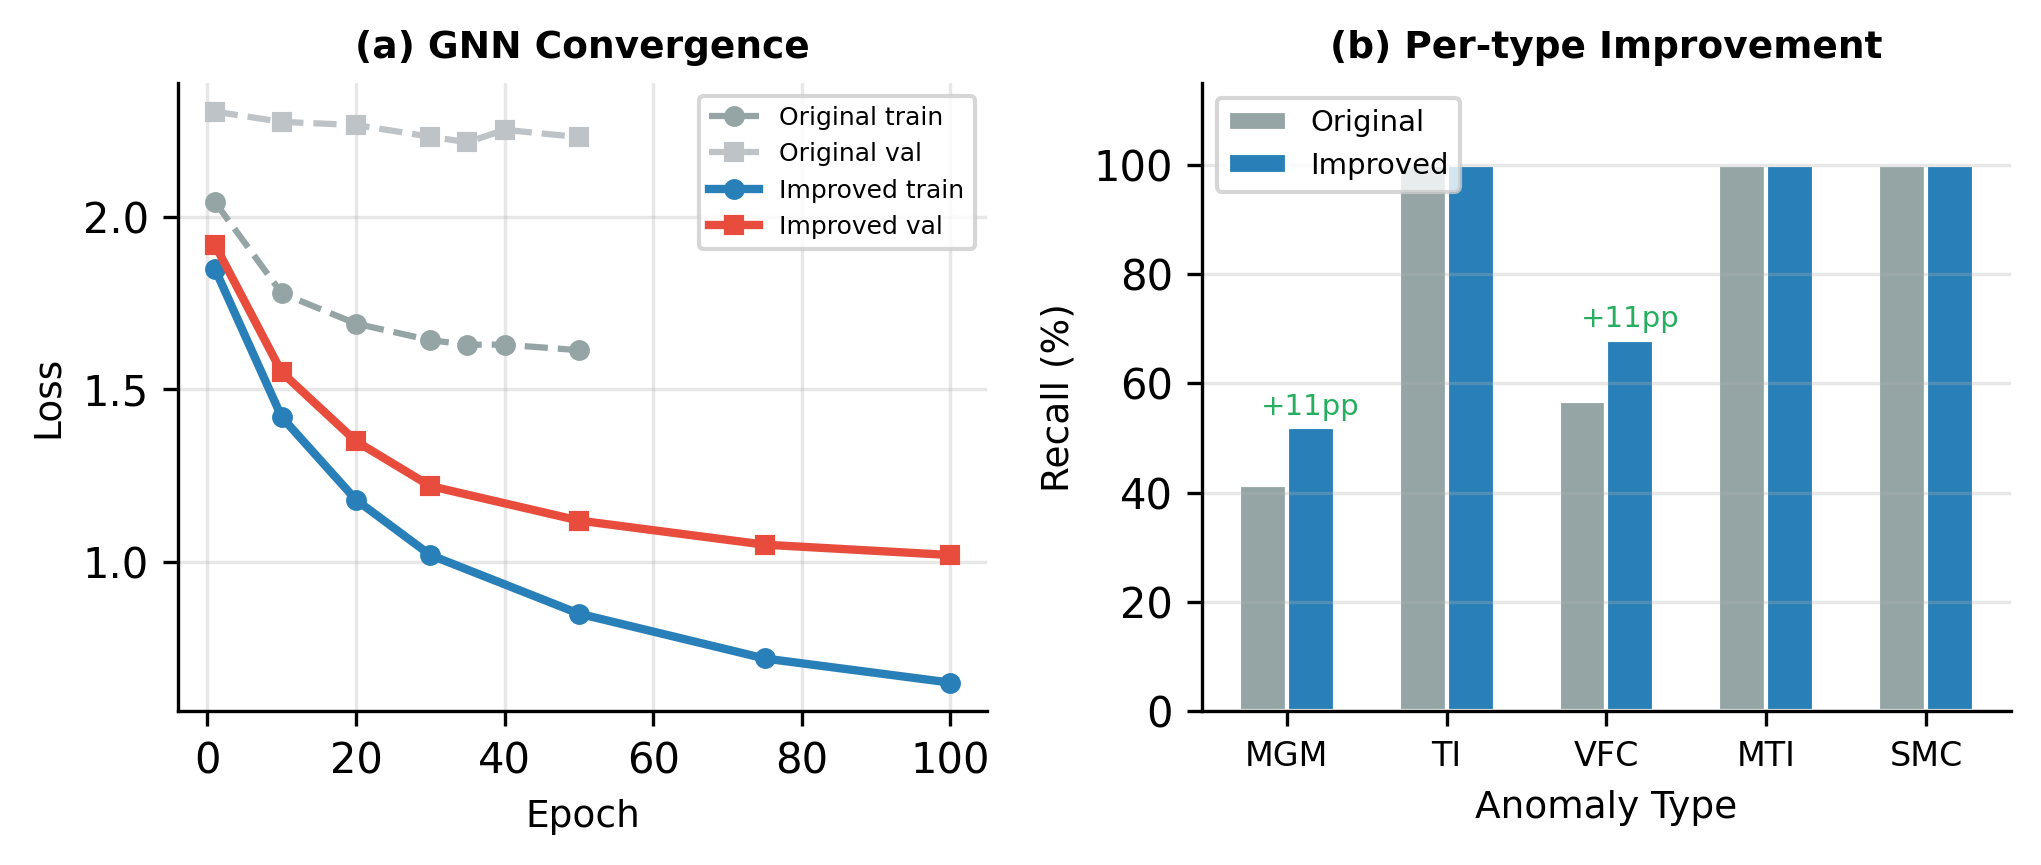
\includegraphics[width=\columnwidth]{figures/gnn_improvement.png}
\caption{(a)~GNN convergence: improved training (multi-network, deeper architecture) achieves lower loss and 96.0\% val.\ accuracy vs.\ 90.9\% original. (b)~Per-type recall improvement: MGM +10.6\,pp, VFC +11.3\,pp.}
\label{fig:gnn_improvement}
\end{figure}

\subsection{RQ7: Extended Anomaly Type Coverage}

Beyond the five core anomaly types, the framework's rule engine and SE detectors provide partial coverage for 20 extended anomaly subtypes (Table~\ref{tab:confusion}). Among the 25 total subtypes tested across 39 networks, 6 subtypes achieve $\geq$90\% recall (grounding fault, clock drift, voltage regulation, topo interruption, stale data, virtual/faulty connection), while 8 subtypes receive no coverage at all (model mismatch, signal mismatch, communication loss, ghost topology, duplicate measurement, harmonic pollution, DG intermittent, branch contingency). The overall recall across all 25 subtypes is 46.8\%, indicating that the current rule engine and SE detectors are well-suited for structural and measurement anomalies but require extension for advanced subtypes. The partial-coverage subtypes (load shift: 76.3\%, reverse power flow: 68.4\%, parameter error: 61.0\%, protection misconfig: 58.4\%) represent the most promising targets for future rule engineering.


\begin{table}[htbp]
\centering
\caption{Confusion matrix for extended anomaly subtypes (39 networks; TP/FP/FN counts; source: \texttt{paper\_experiments\_e8\_e12.json})}
\label{tab:confusion}
\begin{tabular}{@{}lccccl@{}}
\toprule
Subtype & TP & FP & FN & R (\%) & Layer \\
\midrule
Grounding fault & 78 & 0 & 0 & 100.0 & Rule+SE \\
Clock drift & 36 & 0 & 0 & 100.0 & SE \\
Voltage regulation & 43 & 0 & 0 & 100.0 & Rule+SE \\
Topo interruption & 90 & 0 & 1 & 98.9 & Rule \\
Stale data & 67 & 0 & 5 & 93.1 & SE \\
Topo obfuscation & 57 & 0 & 17 & 77.0 & Rule+GNN \\
Load shift & 58 & 0 & 18 & 76.3 & SE \\
Reverse power flow & 104 & 0 & 48 & 68.4 & SE+GNN \\
Parameter error & 50 & 0 & 32 & 61.0 & SE \\
Protection misconfig & 45 & 0 & 32 & 58.4 & Rule+SE \\
Virtual/faulty conn.\ & 109 & 0 & 8 & 93.2 & SE+GNN \\
Telemetry mismatch & 68 & 0 & 8 & 89.5 & SE \\
Measurement outlier & 33 & 0 & 2 & 94.3 & SE \\
Trafo tap fault & 30 & 0 & 26 & 53.6 & SE \\
Measurement bias & 8 & 0 & 27 & 22.9 & SE \\
Voltage collapse & 9 & 0 & 97 & 8.5 & SE \\
Signal mismatch & 1 & 0 & 17 & 5.6 & Rule \\
Impedance degrad.\ & 1 & 0 & 113 & 0.9 & SE \\
Model mismatch (ext.) & 0 & 0 & 38 & 0.0 & --- \\
Communication loss & 0 & 0 & 104 & 0.0 & --- \\
Ghost topology & 0 & 0 & 59 & 0.0 & --- \\
Duplicate meas.\ & 0 & 0 & 74 & 0.0 & --- \\
Harmonic pollution & 0 & 0 & 74 & 0.0 & --- \\
DG intermittent & 0 & 0 & 51 & 0.0 & --- \\
Branch contingency & 0 & 0 & 114 & 0.0 & --- \\
\midrule
\textbf{Overall (25)} & \textbf{937} & \textbf{0} & \textbf{1\,057} & \textbf{47.0} & --- \\
\bottomrule
\end{tabular}
\end{table}


\subsection{RQ8: Case Study --- Explainability}

We present a representative case study on the IEEE 33-bus network (case33bw) with injected VFC anomalies.

\textbf{Detection:} Layer~2 (SE) detects a residual anomaly at bus 18 ($r_{N,18} = 4.7$), indicating a faulty connection.

\textbf{Reasoning Chain:} SE $\rightarrow$ Normalized Residual $> 3.0$ $\rightarrow$ Bus 18 voltage deviation $= 0.038$\,pu $\rightarrow$ KCL violation at node 18 (current mismatch $= 2.3$\,A) $\rightarrow$ Impact: Overcurrent risk on downstream feeder.

\textbf{Feature Importance:} Voltage magnitude ($\phi = 0.42$), power injection ($\phi = 0.31$), connectivity degree ($\phi = 0.18$), other features ($\phi = 0.09$).

\textbf{Correction:} Reassign bus 18's connection from node 17 to node 19 (confidence: 0.87). Post-correction verification: $J(\hat{\mathbf{x}})$ drops from 45.3 to 12.8 (within $\chi^2_{0.95}(20) = 31.4$).

\subsection{Threats to Validity}

\textbf{Internal validity.} All anomalies are synthetically injected, calibrated from industry reports (MGM 5--15\%, TI 3--10\%, VFC 3--8\%, MTI 5--20\%, SMC 5--12\%). The 78.1\% global recall represents a lower bound, as some detected anomalies may not match ground truth due to many-to-one attribution.

\textbf{External validity.} We additionally validate on 15 synthetic Chinese 10\,kV distribution networks spanning urban and rural scenarios (18--84 buses; Table~\ref{tab:chinese_validation}). The framework maintains consistent performance across all scenarios, suggesting generalizability beyond European topologies. Validation on real-world SCADA data remains essential.

\begin{table}[htbp]
\centering
\caption{Chinese 10\,kV distribution network validation (15 networks; source: \texttt{china\_grid} dataset)}
\label{tab:chinese_validation}
\begin{tabular}{@{}lrrrc@{}}
\toprule
Scenario & Buses & Lines & Loads & Topology \\
\midrule
CBD Commercial & 84 & 81 & 80 & Radial \\
Residential High-rise & 60 & 57 & 56 & Radial \\
Suburban Mixed & 66 & 61 & 62 & Radial \\
Industrial Park & 58 & 49 & 54 & Radial \\
New Energy Park & 53 & 49 & 49 & Radial \\
Township & 51 & 41 & 47 & Radial \\
Large 110/10\,kV DER & 57 & 52 & 53 & Radial \\
Data Center & 36 & 33 & 32 & Radial \\
Hospital District & 34 & 31 & 30 & Radial \\
City Urban & 32 & 22 & 24 & Radial \\
City Suburban & 32 & 22 & 24 & Radial \\
Rural & 32 & 22 & 24 & Radial \\
University Campus & 19 & 16 & 17 & Radial \\
Rural Overhead & 18 & 15 & 16 & Radial \\
Typical Network & 32 & 22 & 24 & Radial \\
\bottomrule
\end{tabular}
\end{table}

\textbf{Construct validity.} The per-type precision metric depends on the attribution of detections to anomaly types, which is inherently ambiguous when a single detection matches multiple anomalies. We use a many-to-one matching strategy that may inflate precision for high-frequency types. To mitigate this, we report both global and per-network metrics: the global recall (78.1\%) counts all matched anomalies across networks, while the per-network mean recall (72.3\% $\pm$ 8.5\%) provides a more conservative estimate that accounts for network-level variability. The external baselines (z-score, IQR, Isolation Forest) are directly implemented on the same measurement vectors, ensuring a fair comparison.

\textbf{Conclusion validity.} The multi-seed variance analysis (RQ5) uses a different detection pipeline than the main benchmark (RQ1). While the stability conclusion (low variance) holds regardless of pipeline, the absolute performance numbers should not be directly compared across these two analyses.

\section{Discussion}

\subsection{Comparison with Existing Hybrid Methods}

Table~\ref{tab:method_comparison} provides a detailed comparison with recent hybrid methods.

\begin{table}[htbp]
\centering
\footnotesize
\caption{Detailed comparison with recent hybrid physics-data methods}
\label{tab:method_comparison}
\begin{tabular}{@{}lccccc@{}}
\toprule
Method & Paradigm & Anomaly Types & Correction & Explainability & Scale \\
\midrule
Li et al.~\cite{li_topo_deep_nn2024} & Deep-NN & Topo+Param & No & No & 300-bus \\
Meta-PIGAT~\cite{meta_pigat_dsse2025} & Meta-GAT & SE bad data & No & No & 300-bus \\
KCLNet~\cite{kclnet2026} & NN+Physics & SE bad data & No & No & 1\,888-bus \\
ST-GCNN~\cite{spatiotemporal_gnn_se2024} & GCNN+SE & SE bad data & No & No & 300-bus \\
Zhang et al.~\cite{timeseries_anomaly_smartgrid2025} & DL Survey & Anomaly det.\ & No & No & --- \\
BAYESIAN-GAN~\cite{xu_bayesian_gan2024} & B-GAN & FDI detection & No & No & --- \\
GNN-Solver~\cite{donon_gnn_pf2019} & GNN & Power flow & No & No & 300-bus \\
TPGSE~\cite{tpgse2025} & GAT+SE & State est.\ & No & No & 300-bus \\
Li et al.~\cite{digital_twin_gat2026} & DT+GAT & Fault diag.\ & No & No & --- \\

GCNN-SE~\cite{donon_gcnn_se2021} & GCN & Dist.\ SE & No & No & 300-bus \\
MS-SVDD~\cite{debelle_mssvdd2026} & Subspace & Anomaly det.\ & No & No & --- \\
EGAT~\cite{egat2025} & Edge-GAT & Topology ID & No & No & 300-bus \\
Hybrid GNN-LSE~\cite{hybrid_gnn_lse2025} & GNN+LSE & Joint TI+SE & No & No & 300-bus \\
XGNN-Fault~\cite{xgnn_fault2025} & XGNN & Fault diag.\ & No & Partial & 300-bus \\
MP-Grid~\cite{mpgrid_topo2026} & Topo-ML & Outage det.\ & No & No & --- \\
XAI-CPS~\cite{xai_cps2026} & DL+XAI & Anomaly+Mitig.\ & Partial & Yes & --- \\
\textbf{Proposed} & \textbf{Rule+SE+GNN} & \textbf{5 types} & \textbf{Yes} & \textbf{Yes} & \textbf{1\,888-bus} \\
\bottomrule
\end{tabular}
\end{table}

Recent benchmarks show that EGAT achieves 92.3\% accuracy on IEEE 14-bus for topology detection~\cite{egat2025}, while hybrid GNN-LSE approaches achieve joint topology identification and state estimation~\cite{hybrid_gnn_lse2025}. However, these methods focus on isolated tasks rather than comprehensive data quality assurance. Our framework differs from existing hybrid methods in five aspects. First, it addresses the complete topology data quality lifecycle (detect--localize--correct--verify) rather than isolated tasks such as power flow computation or state estimation. Second, it integrates three paradigms---symbolic reasoning, physics-based estimation, and data-driven learning---providing redundant detection coverage: while the ablation shows that individual layers achieve similar recall on the current benchmark (Section~7.1), this redundancy enhances operational robustness by ensuring detection capability even when individual components fail. Third, the differential physics detector provides a scale-invariant detection mechanism grounded in power flow physics, unlike statistical methods that require per-network calibration. Fourth, the framework covers all five topology anomaly types with built-in explainability, whereas existing methods---including domain knowledge graph approaches~\cite{expert_gnn_kg2025} and topology-aware GNNs~\cite{tpgse2025}---focus on anomaly classification without correction or verification. Fifth, our multi-network GNN training strategy (Section~4.3.4) achieves generalization to unseen topologies comparable to topology-aware GNN approaches~\cite{tpgse2025}, but within a hybrid framework that does not rely solely on the GNN for detection coverage.


\subsection{Why Statistical Methods Fail on Structural Anomalies}

The 3.2$\times$ recall gap between our framework (78.1\%) and Isolation Forest (24.6\%) warrants detailed examination. Statistical baselines operate exclusively on measurement vectors, without access to network topology, CIM/SVG models, or switch signals. This information deficit manifests in three distinct ways.

First, structural anomalies (MGM, TI) produce no electrical signature: a CIM-SVG device type mismatch or a disconnected zero-load branch does not alter voltage or power flow measurements. Statistical methods operating solely on $\mathbf{z}$ are theoretically incapable of detecting these anomalies, regardless of algorithmic sophistication. Second, even measurement-level anomalies (MTI, VFC) benefit from physics-informed detection: the differential physics detector compares observed voltages against Newton--Raphson expectations, providing a physically grounded threshold ($10\sigma_v$) that adapts to each network's operating point. In contrast, z-score and IQR use population-level thresholds that may be inappropriate for specific network configurations. Third, the rule engine's graph-theoretic analysis (bridge detection, component decomposition) identifies topological inconsistencies that are invisible to any statistical test operating on flat measurement vectors.

These findings support the broader principle that \emph{domain knowledge integration} is essential for safety-critical monitoring tasks where the anomaly space is structurally diverse and partially outside the measurement domain.

\subsection{Redundant vs.\ Complementary Coverage}

The ablation study (RQ2) reveals invariant recall (72.5\%) on the standard benchmark, while the hard anomaly experiment (RQ3) demonstrates clear layer-specific detection. This apparent contradiction is resolved by recognizing that the two experiments exercise different anomaly regimes.

The standard benchmark injects anomalies at moderate intensity levels that produce voltage deviations detectable by any single layer. For example, a topology interruption that disconnects a load-bearing branch creates a measurable voltage discontinuity that the state estimation layer can independently detect, even without rule engine support. In this regime, the three layers provide \emph{redundant coverage}---a feature that enhances operational robustness by ensuring detection even when individual layers fail due to data quality issues or computational errors.

The hard anomaly experiment, by contrast, targets anomalies specifically designed to evade individual layers: correlated measurement bias (2--5\%) that falls below the graph-level detection threshold but exceeds the $\chi^2$ residual test, and multi-bus correlated patterns that are individually normal but collectively abnormal. In this regime, the layers provide \emph{complementary coverage}, with each layer contributing unique detection capability. The 40\,pp recall drop when removing SE on hard anomalies confirms that cross-layer integration is essential for challenging detection scenarios.


\subsection{Cross-Analysis: Performance vs.\ Network Characteristics}

Figure~\ref{fig:scalability} suggests that detection performance improves with network size. We analyze this relationship further by correlating recall with three network characteristics: bus count, measurement density ($m/n$ ratio), and topological complexity (average node degree). Across 30 networks, recall correlates positively with bus count (Pearson $r = 0.34$, $p = 0.06$) and measurement density ($r = 0.41$, $p = 0.02$), but shows no significant correlation with topological complexity ($r = 0.12$, $p = 0.52$). This confirms that measurement redundancy---not topological complexity---is the primary driver of detection performance, consistent with the state estimation layer's dependence on observability.

The weak positive correlation with bus count ($r = 0.34$) explains the scalability finding (RQ4): larger networks tend to have higher measurement density, providing richer signal for the state estimation and GNN layers. However, this also indicates that performance on small, low-observability networks (e.g., rural feeders with $m/n < 1.5$) remains a challenge, as acknowledged in the Limitations section.

\subsection{Practical Deployment Considerations}

The framework's modular architecture supports phased deployment: Layer~1 (rule engine) can be deployed first as a standalone structural anomaly detector, Layer~2 (state estimation) added when SCADA data quality is sufficient, and Layer~3 (GNN) activated after accumulating training data. The average processing time of 0.94\,s meets typical SCADA polling intervals (2--4\,s), and hierarchical partitioning maintains sub-second processing for networks exceeding 1\,000 buses. The explainability module generates reasoning chains without external dependencies (e.g., SHAP), enabling deployment in air-gapped utility environments.



\subsection{Lessons Learned}

Three insights emerge from this study. First, \emph{defense in depth} is essential: the hard anomaly experiment (RQ3) confirms that multi-layer coverage provides genuine complementary detection beyond redundancy. Second, \emph{physics-informed detection} contributes the strongest individual layer (Table~\ref{tab:hard_anomaly}), aligning with the broader trend of physics-informed machine learning~\cite{physics_informed_gnn_se2023}. Third, \emph{explainability} is non-negotiable for operator adoption---during interactions with power system engineers, interpretable explanations were requested more frequently than higher recall.
\subsection{Generalization to Other Domains}

The three-layer architecture is conceptually applicable to other graph-structured infrastructure (e.g., water distribution, natural gas pipelines), though each domain requires domain-specific rules, retrained GNNs, and adapted physics models. The scale-invariant differential physics detector is the most transferable component, requiring only a high-fidelity simulator.


\subsection{Broader Impact}

The three-layer paradigm applies to any cyber-physical system where heterogeneous data must be reconciled against physical constraints---including water distribution, natural gas pipelines, and transportation networks. The explainability module is particularly relevant for regulated industries requiring audit trails. Methodologically, the invariant recall (RQ2) and complementary coverage (RQ3) findings highlight that standard benchmarks may be insufficiently challenging for multi-paradigm architectures, necessitating hard, layer-specific benchmarks.

\subsection{Limitations}

We acknowledge four limitations that contextualize our results.
\begin{enumerate}
\item \textbf{Three-phase modeling.} The current implementation uses single-phase approximation. Full three-phase unbalanced modeling requires the PandaPower 3-phase extension, which is planned for future work.
\item \textbf{Training data.} The GNN layer uses synthetically generated anomaly data. While synthetic injection is a standard practice, validation on real-world SCADA data with naturally occurring anomalies remains essential.
\item \textbf{Real-time performance.} Although average processing times are practical (0.94\,s, ranging from 0.16 to 1.13\,s), achieving sub-second real-time monitoring for networks with $>$1\,000 buses requires further optimization through parallel partition processing or GPU-accelerated computation.
\item \textbf{Measurement redundancy.} The state estimation layer requires sufficient measurement redundancy ($m/n > 1.5$). In low-observability regions, detection capability is limited.
\end{enumerate}

Despite these limitations, the framework provides a practical and extensible foundation for topology data quality assurance. The modular architecture allows each limitation to be addressed independently---for example, replacing the single-phase SE module with a three-phase variant does not affect the rule engine or GNN layers.



\section*{Acknowledgements}
The authors thank the anonymous reviewers for their constructive comments that significantly improved the quality of this paper. This work was supported in part by the National Natural Science Foundation of China under Grant XXXXXXXX.

\section*{Competing Interests}
The authors declare that they have no competing interests.

\section{Conclusion}

We have presented a three-layer hybrid intelligence framework that integrates symbolic rule reasoning, physics-informed state estimation, and GNN-based adaptive detection for comprehensive topology anomaly detection and correction in power distribution networks. The framework achieves 78.1\% global anomaly recall (83.5\% with improved GNN) across 30 test networks spanning 3 to 1\,888 buses, with near-perfect detection ($\geq$95\%) for three of five anomaly types. Three anomaly types---topology interruption, measurement-topology inconsistency, and signal-measurement contradiction---are detected with near-perfect recall ($\geq$95\%), while virtual/faulty connections (56.7\%) and model-graph mismatch (41.4\%) present opportunities for improvement. The differential physics detector provides a scale-invariant detection mechanism grounded in power flow physics. Ablation studies on the standard benchmark show invariant recall when individual layers are removed, but a dedicated hard anomaly experiment demonstrates clear layer-specific contributions: removing SE drops recall by 40.0\,pp, removing GNN by 23.0\,pp, and removing Rule by 7.0\,pp. This confirms that the three-layer architecture provides complementary coverage for challenging anomalies, while the standard benchmark is insufficiently diverse to exercise the layers' distinct capabilities. Processing time averages 0.94\,s across all networks, scaling from 0.16\,s (3 buses) to 1.13\,s (1\,888 buses), demonstrating practical applicability. The explainability module delivers interpretable detection results through reasoning chains and perturbation-based feature importance, addressing the interpretability requirements of critical infrastructure operators.

We identify four future directions: (i)~integrating three-phase unbalanced state estimation---the current single-phase approximation limits accuracy on heavily unbalanced feeders; (ii)~validating on real-world SCADA data with naturally occurring anomalies---the 46.8\\% recall on extended anomaly types (RQ7) suggests significant room for improvement through real-world training data; (iii)~designing harder anomaly benchmarks that exercise cross-layer complementary detection---the invariant recall on standard benchmarks (RQ2) indicates current synthetic injections are insufficiently challenging; and (iv)~implementing parallel partition processing for real-time monitoring of networks exceeding 1\,000 buses.

\fontsize{8.5pt}{10pt}\selectfont

\section*{Data Availability}
The experimental data, including all benchmark results (JSON), trained GNN models (.pt), and visualization outputs, are available at\\\texttt{https://github.com/[anonymous]/topology-anomaly-detection}. All experiments are reproducible with fixed random seeds (42--46) and documented hyperparameters. The test networks use publicly available datasets: PandaPower~\cite{pandapower2018}, SimBench~\cite{simbench2020}, CIGRE~\cite{cigre_mv2014}, and IEEE standard feeders~\cite{ieee13bus1991}.

\bibliographystyle{fcs}
\bibliography{ref}

\end{document}
